%thesis.tex
%Model LaTeX file for Ph.D. thesis at the
%School of Mathematics, University of Edinburgh

\documentclass[10pt,twoside,openright,logo]{report}

\title{A Profiling Mechanism for dispel4py}
\author{Anqi Lu}
\date{2015}

\usepackage[msc]{edmaths}
\usepackage{graphicx}
\usepackage{xcolor}
\usepackage{dirtree} % Used for diretory tree drawing
% The following is a dummy icon command
\newcommand\myicon[1]{{\color{#1}\rule{2ex}{2ex}}}
% If you have actual icon images, use \includegraphics to include them
% If you are generating them, put in the appropriate code for them here
% now we make a command for a folder/file which inserts the icon and its label
% adjust this as needed. If you only have 2 icons, then you could create
% a \myfile and \myfolder command with the icon fixed.
\newcommand{\myfolder}[2]{\myicon{#1}\ {#2}}

\usepackage{minted} % Used for syntax highlight and verbatim

\usepackage{mathtools} % Used for displaying math notations

\usepackage{amsmath} % Used for dispalying nice looking fractions with text

\usepackage[framemethod=default]{mdframed} % Used for contain contents with frame

\mdfsetup{nobreak=true, align=center}
\surroundwithmdframed{minted}

\usepackage{adjustbox} % Used for page fit

\usepackage{graphicx} % Importing graphics

\usepackage{seqsplit} % Split long sequence in any location

\graphicspath{{images/}{../images/}}
\begin{document}
%%% Claim Figure Here %%%
\def\figone{%
    \begin{figure*}[!htb]
        \centering
        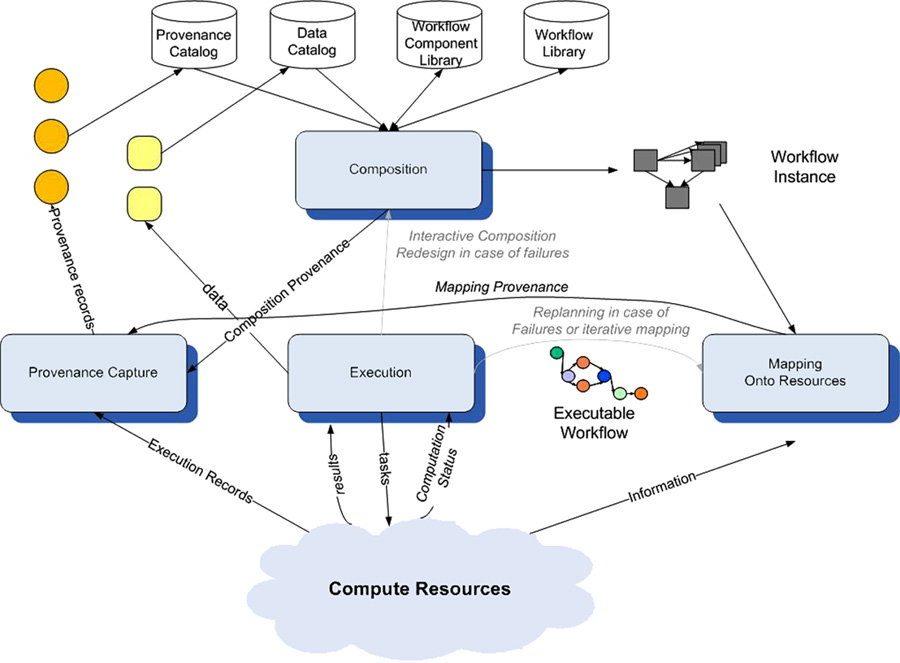
\includegraphics[width=0.9\textwidth]{figure-1}
        \caption{The workflow lifecycle: composition, mapping, execution, and provenance capture (Deelman, E. 2009)
                \label{fig:one}
                }
    \end{figure*}
\global\let\figone\relax}

\def\figtwo{%
    \begin{figure*}[!htb]
        \centering
        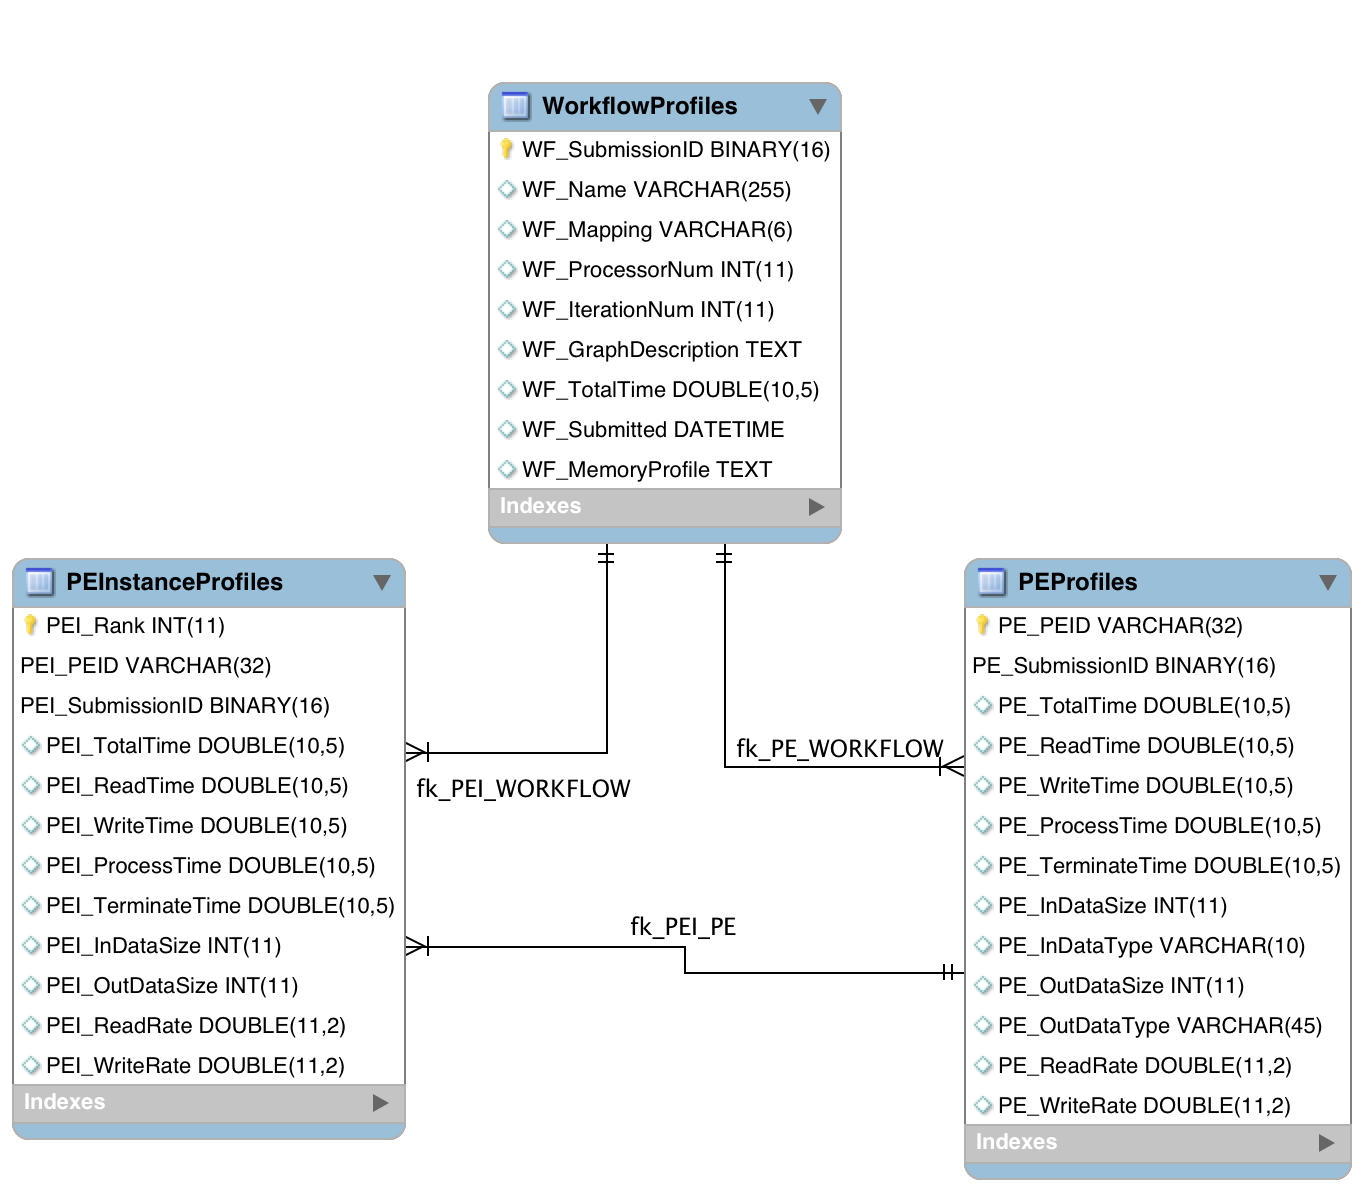
\includegraphics[width=0.9\textwidth]{figure-2}
        \caption{The enhanced entity–relationship (EER) model of relational performance data in MySQL database
                \label{fig:two}
                }
    \end{figure*}
\global\let\figtwo\relax}

\def\figthree{%
    \begin{figure*}[!htb]
        \centering
        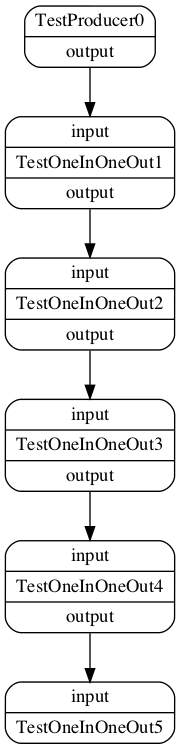
\includegraphics[scale=0.5]{figure-3}
        \caption{The graph of PipelineTest, a pipeline workflow with 1 producer and 5 consumers
                \label{fig:three}
                }
    \end{figure*}
\global\let\figthree\relax}

\def\figfour{%
    \begin{figure*}[!htb]
        \centering
        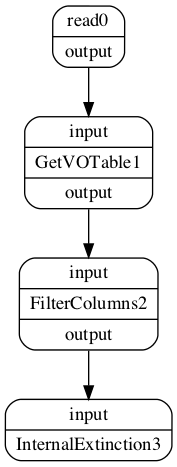
\includegraphics[scale=0.5]{figure-4}
        \caption{The graph of Internal Extinction of Galaxies (Astro), a pipeline workflow with 1 producer and 3 consumers
                \label{fig:four}
                }
    \end{figure*}
\global\let\figfour\relax}

\def\figwf{%
    \begin{figure*}[!htb]
        \centering
        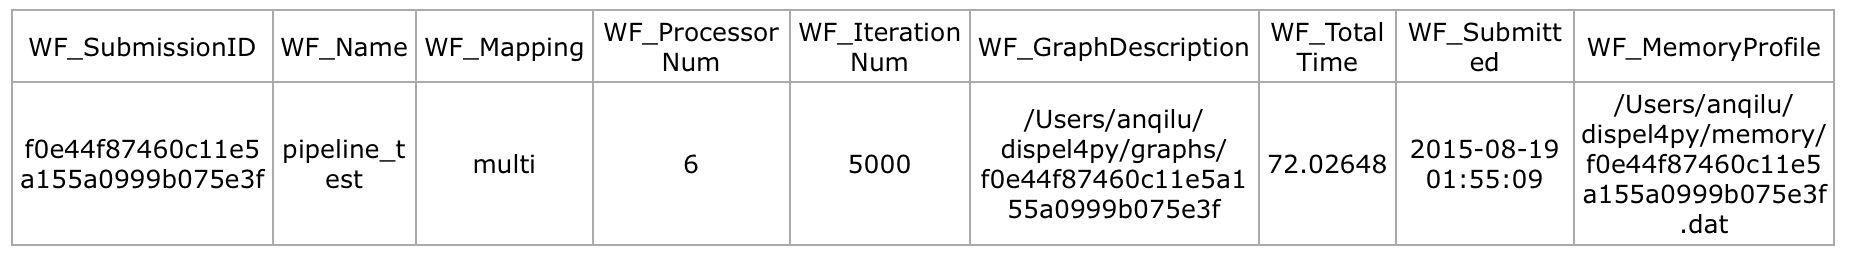
\includegraphics[width=\textwidth, keepaspectratio]{pip-wf}
        \caption{Characteristics of workflow captured from Pipeline Test, stored as WorkflowProfiles in MySQL database
                \label{fig:pip-wf}
                }
    \end{figure*}
\global\let\figwf\relax}

\def\figpe{%
    \begin{figure*}[!htb]
        \centering
        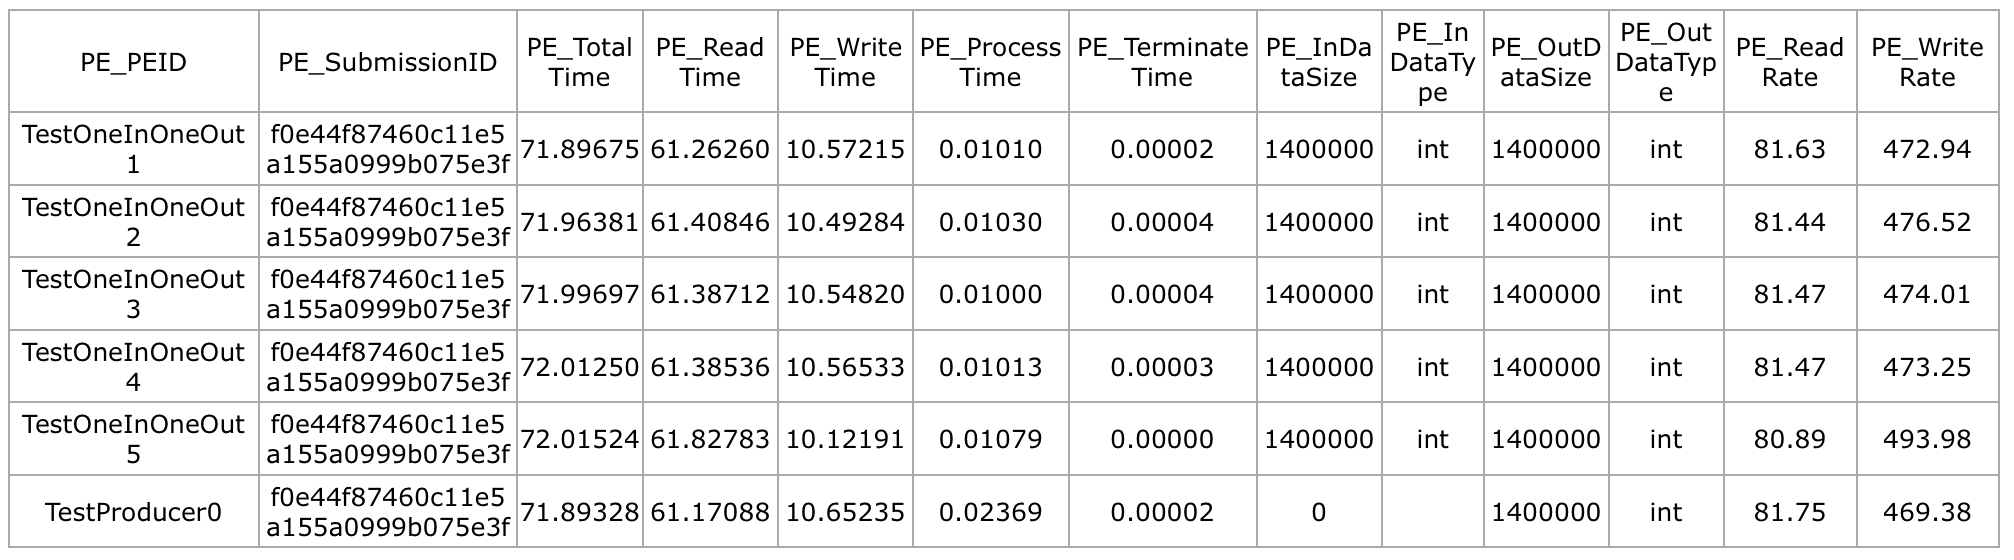
\includegraphics[width=\textwidth, keepaspectratio]{pip-pe}
        \caption{Characteristics of PE captured from Pipeline Test, stored as PEProfiles in MySQL database
                \label{fig:pip-pe}
                }
    \end{figure*}
\global\let\figpe\relax}

\def\figpei{%
    \begin{figure*}[!htb]
        \centering
        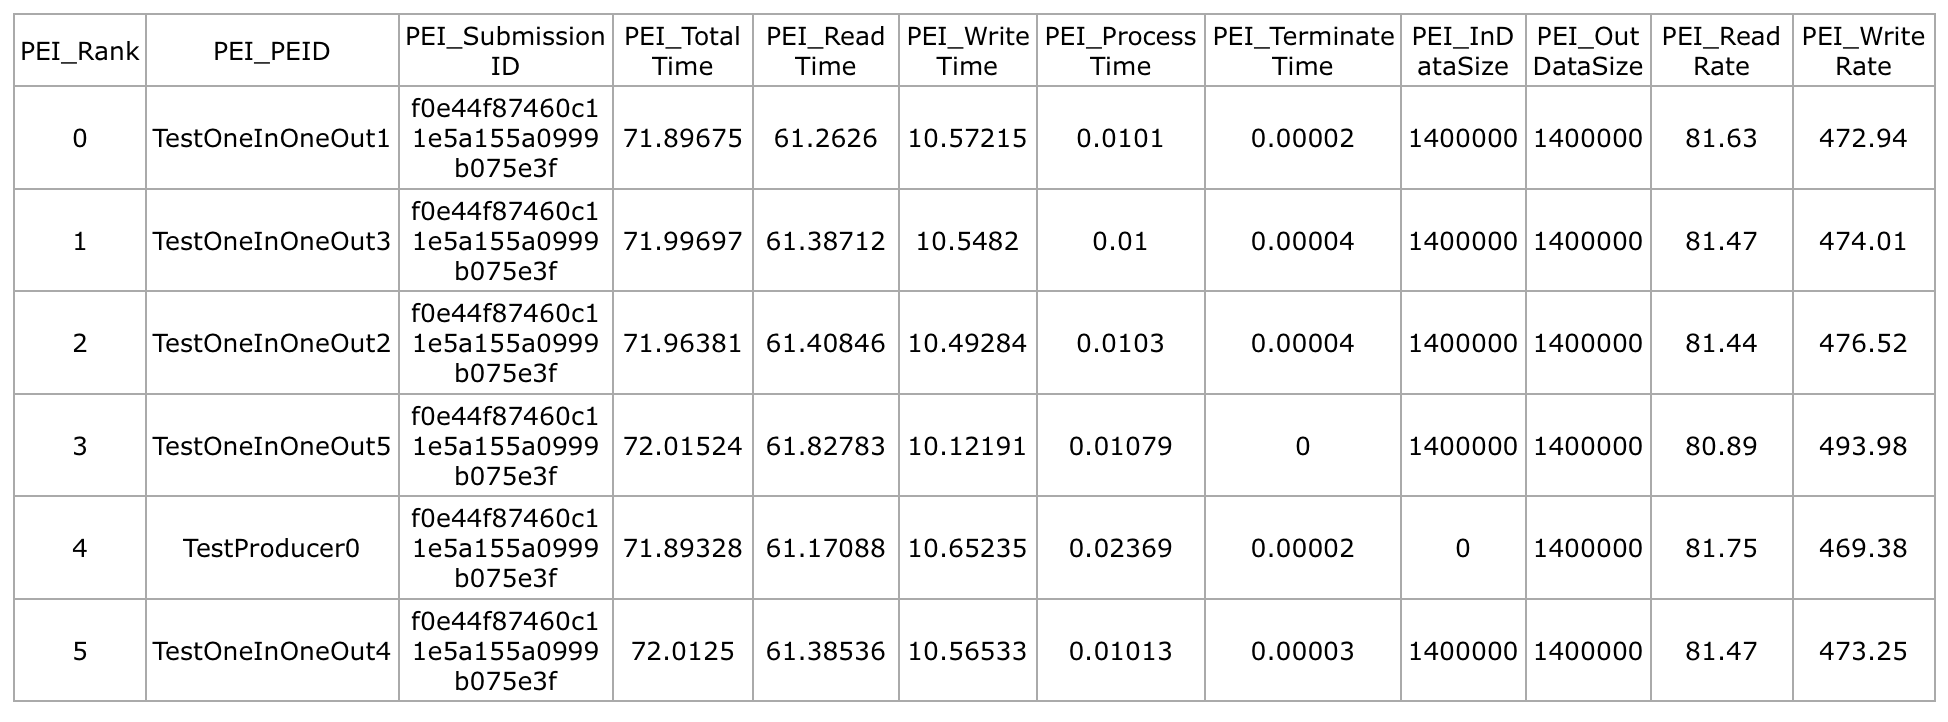
\includegraphics[width=\textwidth, keepaspectratio]{pip-pei}
        \caption{Characteristics of PEI captured from Pipeline Test, stored as PEInstanceProfiles in MySQL database
                \label{fig:pip-pei}
                }
    \end{figure*}
\global\let\figpei\relax}

\def\figastropt{%
    \begin{figure*}[!htb]
        \centering
        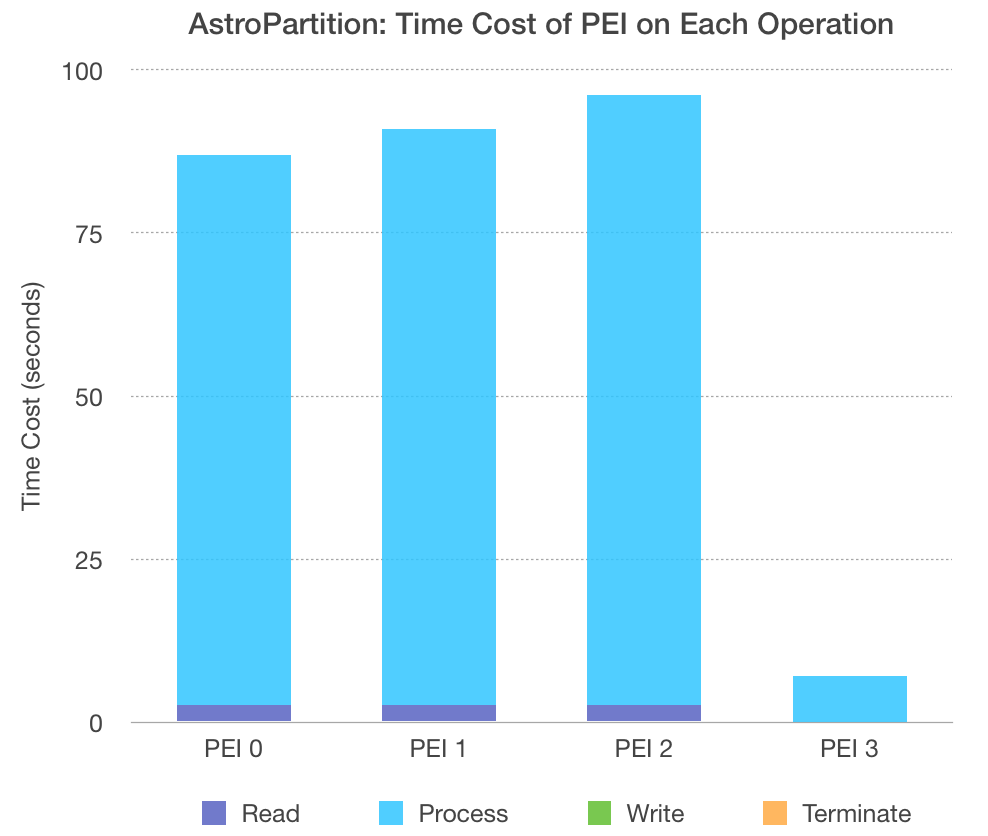
\includegraphics[scale=0.5]{figure-astrop-t}
        \caption{Time cost of each four operations of four PEIs in AstroPartition
                \label{fig:astrop-t}
                }
    \end{figure*}
\global\let\figastropt\relax}

\def\figastroit{%
    \begin{figure*}[!htb]
        \centering
        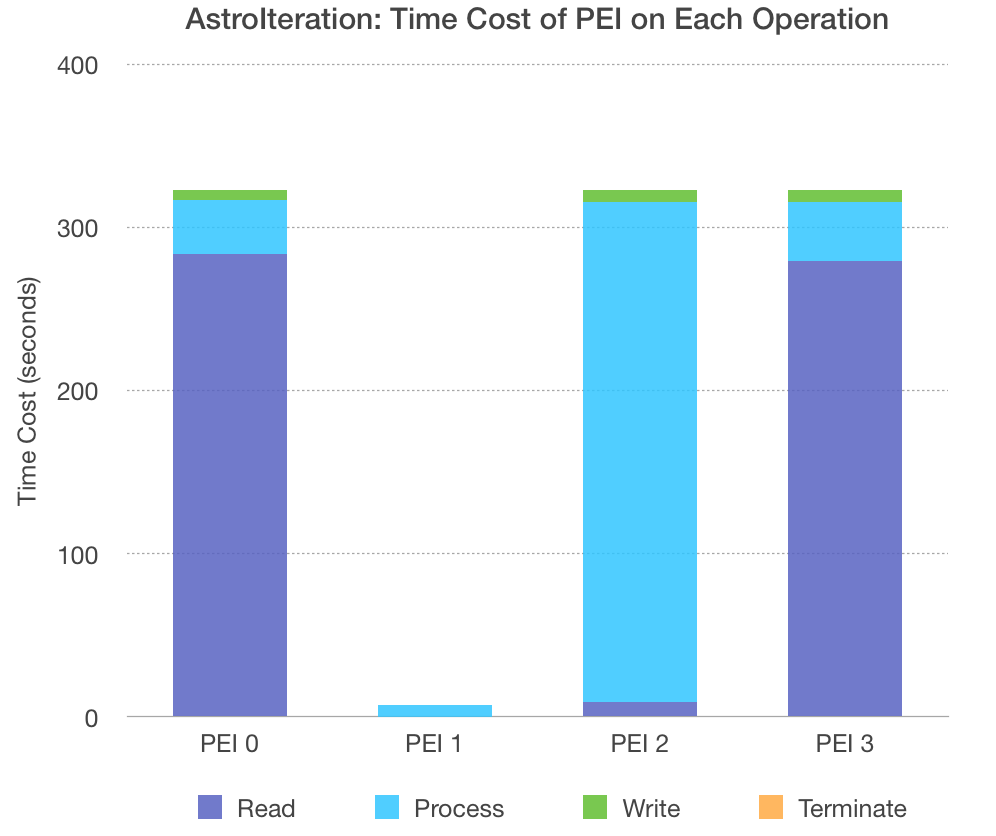
\includegraphics[scale=0.5]{figure-astroi-t}
        \caption{Time cost of each four operations of four PEIs in AstroIteration
                \label{fig:astroi-t}
                }
    \end{figure*}
\global\let\figastroit\relax}

\def\figastropx{%
    \begin{figure*}[!htb]
        \centering
        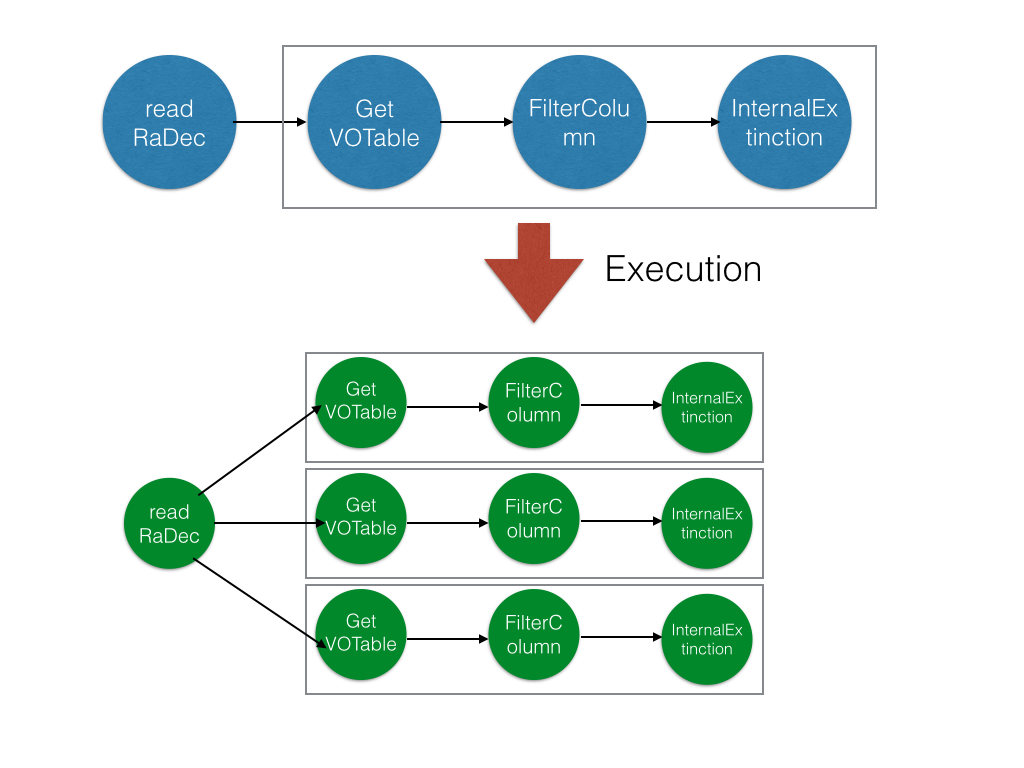
\includegraphics[scale=0.2]{figure-astrop-exec}
        \caption{Enact Astro workflow in a partitioned manner (AstroPartition)
                \label{fig:atrop-exec}
                }
    \end{figure*}
\global\let\figastropx\relax}

\def\figastroix{%
    \begin{figure*}[!htb]
        \centering
        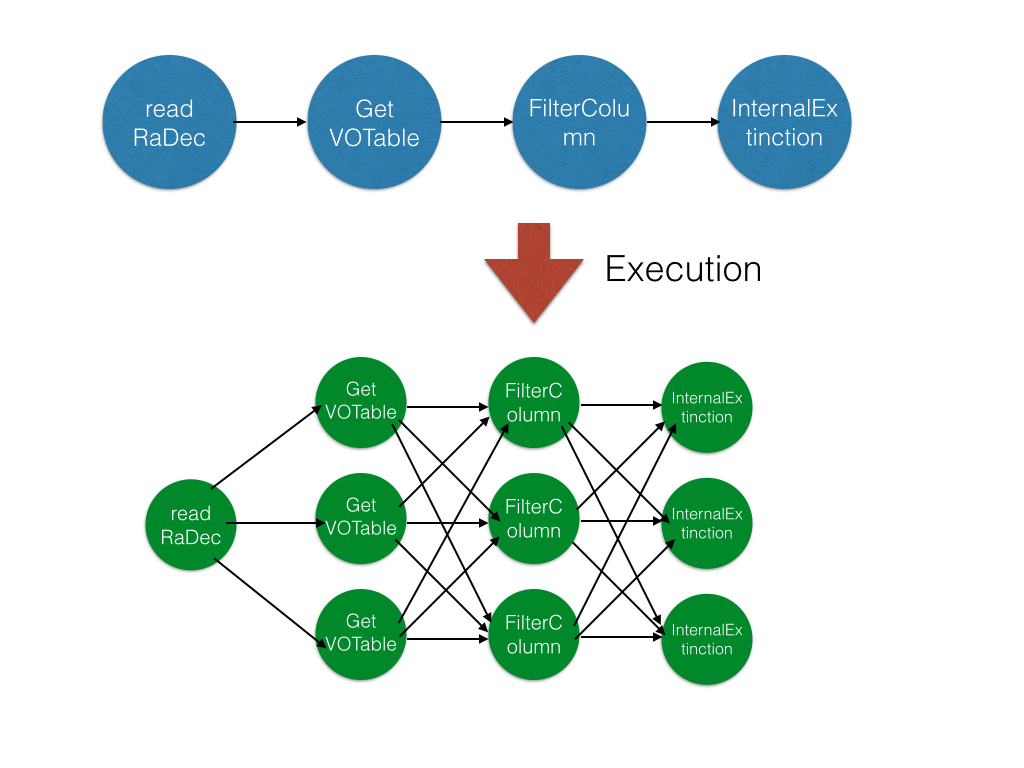
\includegraphics[scale=0.2]{figure-astroi-exec}
        \caption{Enact Astro workflow in a common iterative manner (AstroIteration)
                \label{fig:atroi-exec}
                }
    \end{figure*}
\global\let\figastroix\relax}

\def\figaspzero{%
    \begin{figure*}[!htb]
        \centering
        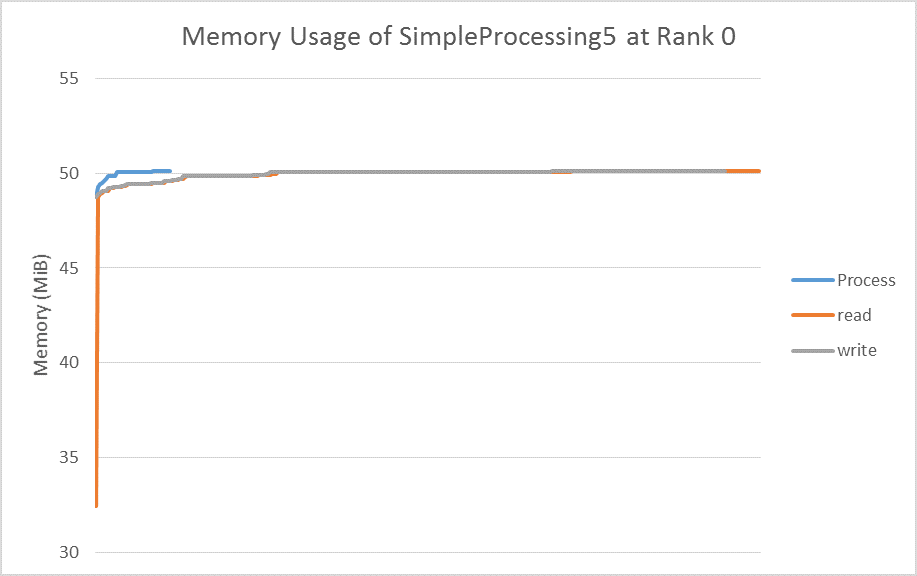
\includegraphics[scale=0.5]{mem-0}
        \caption{During enactment of AstroPartition, the memory usage trend of SimpleProcessing5 at rank 0 process
                \label{fig:atrop-zero}
                }
    \end{figure*}
\global\let\figaspzero\relax}

\def\figaspone{%
    \begin{figure*}[!htb]
        \centering
        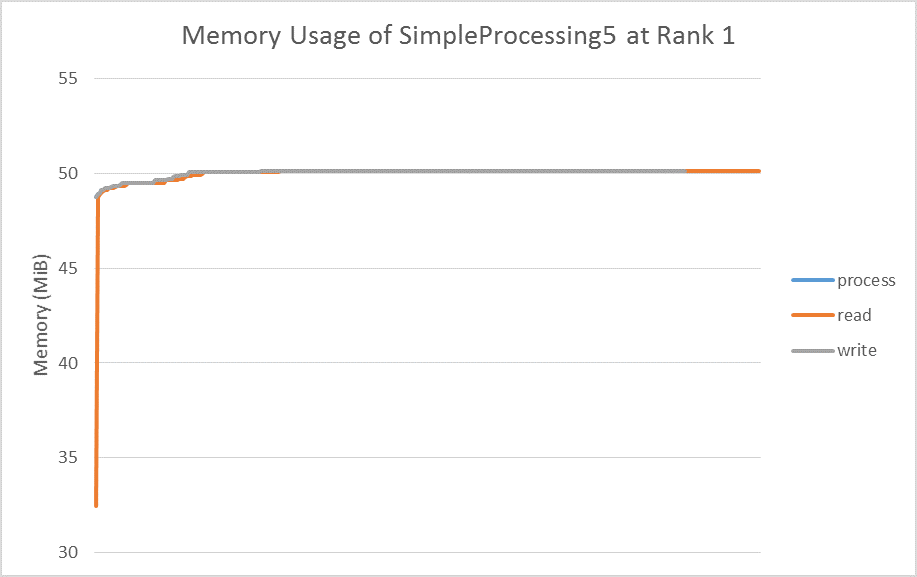
\includegraphics[scale=0.5]{mem-1}
        \caption{During enactment of AstroPartition, the memory usage trend of SimpleProcessing5 at rank 1 process
                \label{fig:atrop-one}
                }
    \end{figure*}
\global\let\figaspone\relax}

\def\figasptwo{%
    \begin{figure*}[!htb]
        \centering
        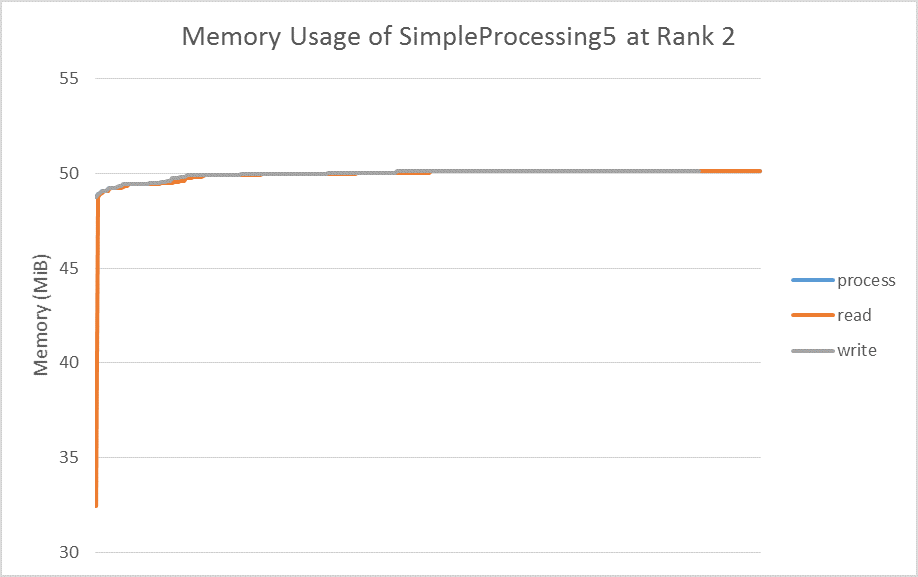
\includegraphics[scale=0.5]{mem-2}
        \caption{During enactment of AstroPartition, the memory usage trend of SimpleProcessing5 at rank 2 process
                \label{fig:atrop-two}
                }
    \end{figure*}
\global\let\figasptwo\relax}

\def\figaspthree{%
    \begin{figure*}[!htb]
        \centering
        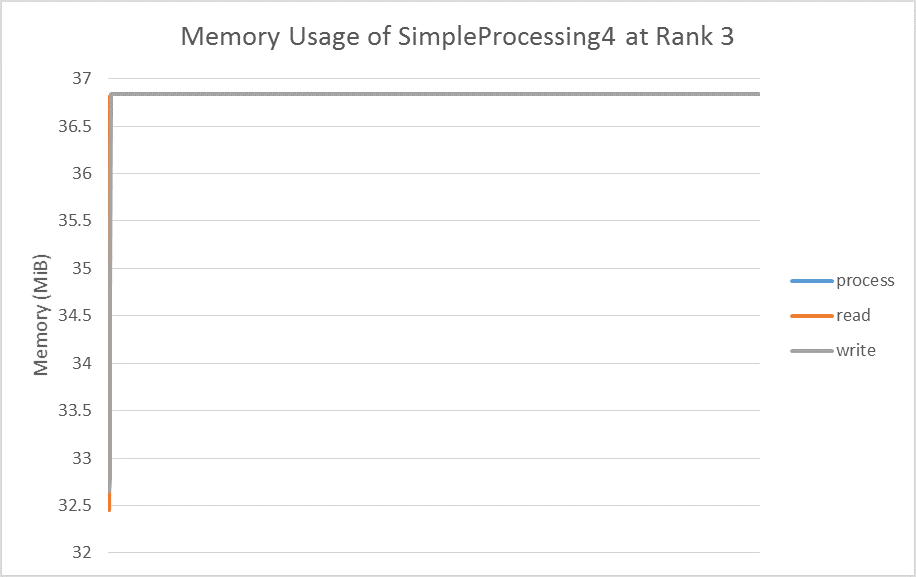
\includegraphics[scale=0.5]{mem-3}
        \caption{During enactment of AstroPartition, the memory usage trend of SimpleProcessing4 at rank 3 process
                \label{fig:atrop-three}
                }
    \end{figure*}
\global\let\figaspthree\relax}

\def\figmemtwoa{%
    \begin{figure*}[!htb]
        \centering
        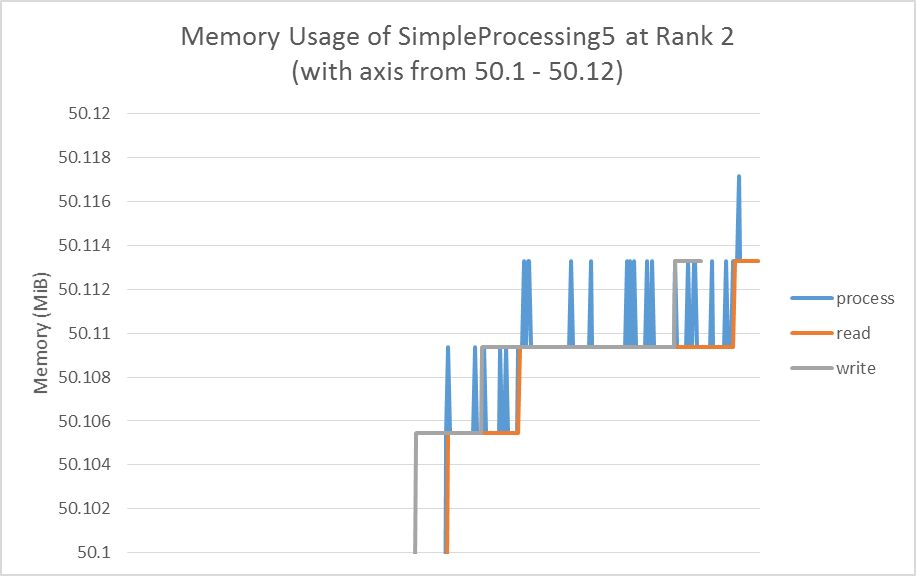
\includegraphics[scale=0.5]{mem-2-a}
        \caption{During enactment of AstroPartition, the memory usage trend of SimpleProcessing5 at rank 2 process, from 50.1 - 50.12 MiB
                \label{fig:astrop-memtwoa}
                }
    \end{figure*}
\global\let\figmemtwoa\relax}

\def\figmemtwob{%
    \begin{figure*}[!htb]
        \centering
        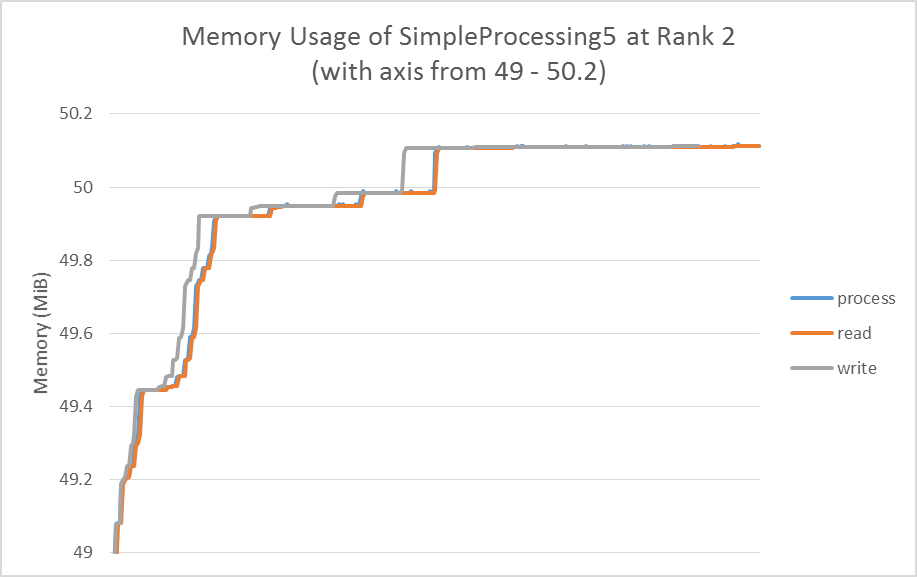
\includegraphics[scale=0.5]{mem-2-b}
        \caption{During enactment of AstroPartition, the memory usage trend of SimpleProcessing5 at rank 2 process, from 49 - 50.2 MiB
                \label{fig:astrop-memtwob}
                }
    \end{figure*}
\global\let\figmemtwob\relax}

\def\figastroim{%
    \begin{figure*}[!htb]
        \centering
        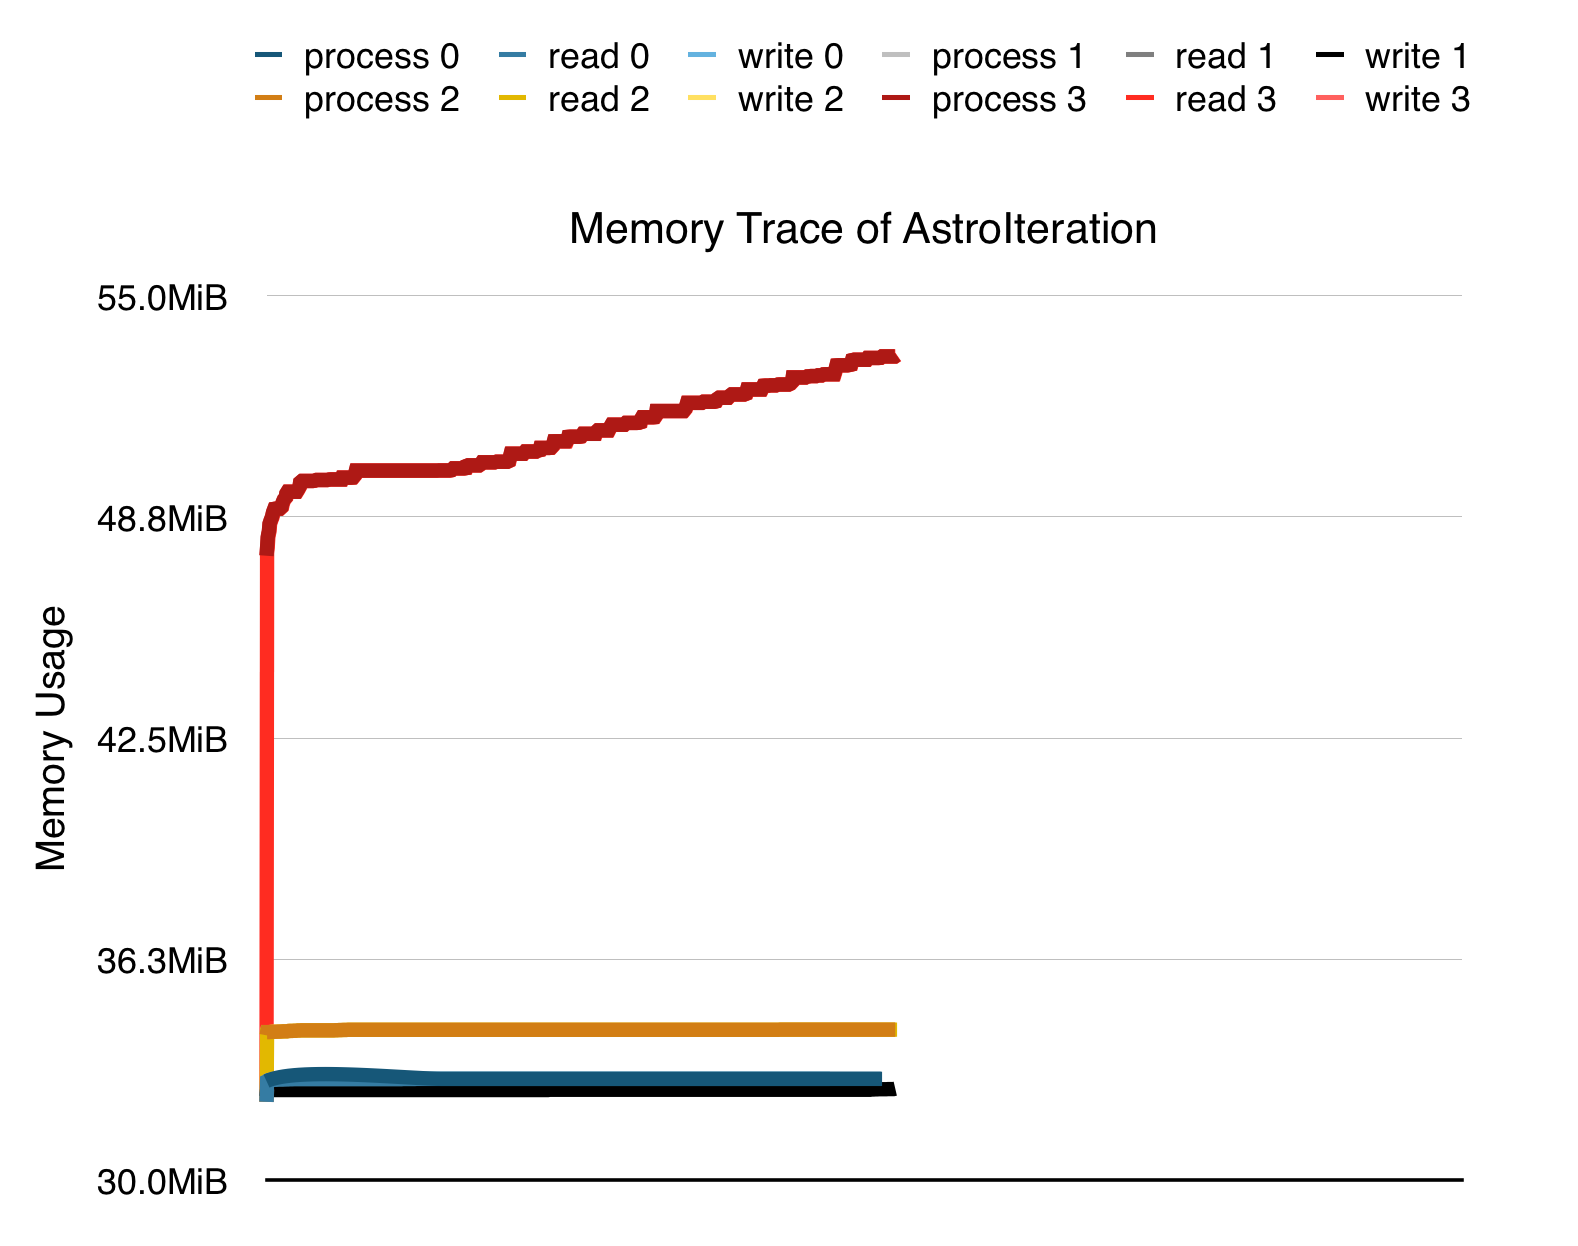
\includegraphics[scale=0.5]{figure-astroi-mem}
        \caption{During enactment of AstroIteration, the memory usage trend of PEIs on process, write and read
                \label{fig:astroi-memzero}
                }
    \end{figure*}
\global\let\figastroim\relax}

\def\figastrocomp{%
    \begin{figure*}[!htb]
        \centering
        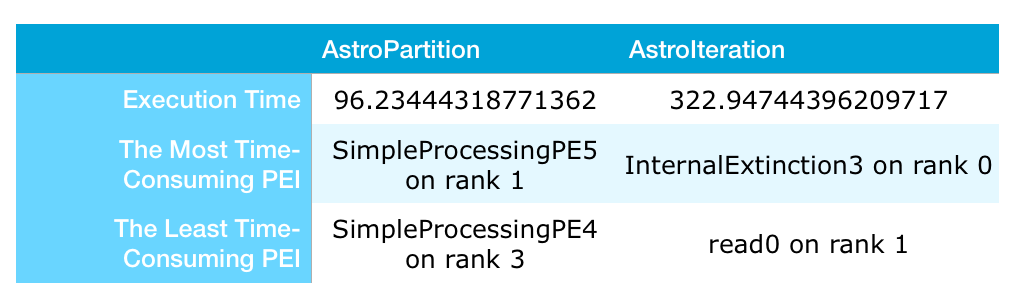
\includegraphics[scale=0.5]{figure-astro-comp}
        \caption{ Comparison between AstroPartition ans AstroIteration
                \label{fig:astro-comp}
                }
    \end{figure*}
\global\let\figastrocomp\relax}
\maketitle

\declaration

\dedication{To everybody I met here in Edinburgh.}

\begin{abstract}
\noindent This project built an infrastructure to profile performance of dispel4py workflows. The profiling mechanism consists of profiling framework (PF) and performance database (PDB). PF captures workflow characteristics (i.e. timings, memory, data stream properties, topology of workflow), and organizes raw data before permanently store it. Then PF flushes processed data to PDB, which manages memory, topology of workflow and other characteristics respectively. Future analysis on the historical data can be made on PDB to improve the efficiency of dispel4py workflows. This profiling infrastructure now works in the Multi-Processing distributed computational infrastructure. To illustrate the usage and value of this mechanism, Pipeline Test workflow and Internal Extinction of Galaxies workflow were profiled and analyzed.
\end{abstract}

\tableofcontents

\chapter{Introduction}
Data-intensive computing, assumed as the fourth Paradigm\cite{8}, is getting its popularity in many research fields these days. Such computational applications involve a large volume of data when enacting and spend most of processing time on I/O and manipulation of data. As a result of growing applications of data-intensive computing, heterogeneity, scale and complexity of data involved in scientific research increase fast. Consequently, to automatically handle the low-level data processing, scientific workflow systems emerge. Scientific workflow systems allow scientists to focus on high-level infrastructure (i.e. logical level of computations) rather than being distracted by implementation details of a computation on distributed systems\cite{9}.

The performance data of scientific workflows and scientific workflow systems helps researchers to better understand the workflow enactments in practice. It can be examined for errors and exceptional behaviors, analyzed for optimization, mined and processed for a profile of a certain workflow.

dispel4py\cite{1} is a novel scientific workflow system, which translate abstract workflow graphs into a couple of mappings, including Apache Storm, MPI, shared-memory Multi-Processing and Sequential Mode. It enables users to use a fine-grained workflow to describe computational tasks. Additionally, dispel4py streams data in the graph, which avoids writing intermediate values to disk except when buffers overflow RAM.

This dissertation presents a profiling mechanism for dispel4py workflow system in multi-processing distributed environment. The goal is to profile each computational block of a workflow in following aspects: time cost, memory occupation and data stream properties (i.e. data stream rate, data size, data type). Performance data is captured and processed by profiling framework (PF) , an infrastructure to track runtime workflows. Then, raw data collected from intercepting certain parameters is gathered and used to build a performance database (PDB) . Further study is made in the characterization statistics for learning about the workflows. To illustrate an implementation of the profiling mechanism, benchmark profiles were built for two workflows, \textit{Pipeline Test} workflow and \textit{Internal Extinction of Galaxies} workflow, working with Multi-Processing mapping, on local server and clusters, respectively.

%------------------------------------------------

\chapter{Background}
\figone
\section{Scientific Workflows}
As complex and vast computations are developing rapidly, there emerge requirements for computation management. Specifically, imagine there is a bunch of repetitive operations involving inputting data to a supercomputer, a sequence of processing on data, and outputting data to somewhere. Apparently, it requires automatic management for the movement of the data and the control of the repetitive cycle. This is exactly the purpose of scientific workflow systems, which aims at automating this cycle to enable scientists focus on algorithms or services themselves instead of computation infrastructure\cite{2}.

There are a couple of concepts to clarify about \textit{workflow}:

\textit{Workflow Orchestration} refers to the activity of defining the sequence of tasks needed to manage a business or computational science or engineering process.

A \textit{Workflow} is a template for such an orchestration.

A \textit{Workflow Instance} is a specific instantiation of a workflow for a particular problem and includes the definition of input data.

A workflow is made up of a set of tasks and dependencies between each task. Furthermore, the dependencies between tasks must be satisfied to ensure the workflow work as expected. As is said in \cite{4}, the goal of e-Science workflow systems is to provide a specialized programming effort required by scientists to orchestrate a computational science experiment. That is also the aim of dispel4py, which is the e-Science workflow system being studied in this paper and will be introduced in the next subsection.

As is illustrated in Figure \ref{fig:one}, the lifecycle of a workflow can be classified as four phases:
\begin{enumerate}
    \item \textbf{Composition:}
    Certain workflow is defined in this phase by users. The composition phase allows the specification of steps and dependencies of a workflow.

    Workflows can be described either directly or with a template. In the former case, users specify a workflow with computational steps and the specific data. In contrast, in the latter case, users first create a template and then instantiate it with actual data.

    Depending on the level of composition tasks, workflow systems can be classified as task-based or service-based. Task-based systems focus on the resource-level features, leaving higher-level tasks to other tools, while service-based ones provide interfaces to certain classes of service for management and composition.

    \item \textbf{Mapping:}
    In this phase, the description, created in the previous phase, is used to build an executable workflow.

    Both task-based systems and service-based systems involve finding necessary resources/ services to execute computation, and optimization. Moreover, task-based systems may modify the original workflow in this phase.

    \item \textbf{Execution:}
    The workflow is executed in this phase.

    \item \textbf{Provenance:}
    Data provenance refers to a record of the history of the creation of a data object.

\end{enumerate}

\section{dispel4py}
dispel4py\cite{1} is a Python library used to describe abstract workflows for distributed data-intensive applications. Data-intensive applications refer to applications that are I/O bound or with a need to process large volumes of data\cite{3}. Due to the size of input data, the processing time of these specific applications is mostly consumed at the following phases: data input, data movement, data manipulation, and data output.

The purpose of dispel4py is to enable users to implement manipulations on big data without being distracted by details of the computing framework. To achieve this, dispel4py works in a dataflow-oriented way. With data streaming, it therefore can process requests with large-scale data by an efficient implementation of buffering in the main memory where the processing speeds of memory access outperform the disk by a factor of more than $10^5$ \cite{10}. Dispel4py workflow can be viewed as a light-weight composition of data operations. Data is streamed from one computational operation to another. That means any intermediate I/O cost is avoided.

Dispel4py instantiate workflow with a \textit{graph} customized by users. A graph defines the ways in which computational blocks are connected and hence the paths taken by data, i.e. the topology of the workflow. A \textit{processing element} (PE) can be assumed as a basic computational block, which encapsulates an algorithm, a service or another data transformation process. It allows users to describe their tasks in each PE in Python script and then define the connections of each PE, which is called graph. In a workflow, each PE is connected with data stream. A \textit{processing element instance} (PEI) is the executable copy of a PE instantiated in runtime workflow.

According to different infrastructure of workflows, there are four types of PEs, which are composed of \textit{generic PE}, \textit{iterative PE}, \textit{simple function PE} and \textit{iterative chain}. Generic PE allows multiple input data flows and multiple output data flows while the others just allow single input and single output. The compositions of a variety of PEs in a graph enables the merging and splitting of data streams as desire. Additionally, different PEs can be composed together to form a \textit{composite PE}, which allow for synthesis of increasingly complex workflows. In parallel environment, a dispel4py \textit{partition} refers to several PEs running in a single process.

dispel4py currently supports following mappings: Apache Storm, MPI, Multi-Processing and Sequential Mode.
Apache Storm is a distributed realtime computation system. The dispel4py system maps to Storm by translating its graph description to a Storm topology.
MPI, Message Passing Interface, is a standardized and portable message-passing system. dispel4py uses mpi4py, a Python binding for MPI based on the MPI-2 standard to map PEs to a collection of MPI processes.
Compared with message passing model, Multi-Processing, a Python package that supports spawning processes, works in a memory sharing way to commit parallel tasks.
Sequential mode (simple) is a standalone mode that is ideal for small applications running on local server.
The first three mappings are designed for distributed resources while the last one acts as baseline for workflow development.
The performance profiling and evaluation in this project is mainly focused on Multi-Processing.

\section{Related Work on Profiling Scientific Workflows}
Many efforts have been made in the study of scientific workflow profiling. An workflows profiling method was introduced in \cite{5}. Juve and Chervenak developed \textit{wfprof}, a workflow characterization tool-kit, to record and analyse performance metrics for workflows. The workflow parameters studied in this research were composed of process I/O, runtime, memory and CPU (Central Processing Unit) utilization. In \cite{2}, a taxonomy was proposed to characterize and classify methods for enacting workflows in Grid computing. Callaghan et al. proposed a novel method to accurately capture the scale of scientific workflows and quantify their efficiency in \cite{4}. Detailed task-level characterization was studied in their research. Profiles built from historical enactments of workflows could be used in optimization of future workflows along with scheduling algorithms \cite{6}.

Performance database was introduced by Liew et al. in \cite{7}. A performance database (PDB) refers to a database storing performance-related data gathered during workflow enactment. To describe how performance data is collected and transformed into information, a four-stage lifecycle (collect, organize, use and discard) was introduced in this paper. The concept of PDB in our study is different with what they proposed. PDB is permanently stored on our disk instead of being discarded after analysis. This enables further usage on the history performance data for workflows working in the similar conditions, such as topology of the workflow network.

%------------------------------------------------

\chapter{dispel4py Performance Profiling Mechanism}
\section{Overview on Performance Profiling Mechanism}
dispel4py performance profiling mechanism is designed for better understanding the efficiency of enactments of workflows, and optimizing it. In terms of architecture, it consists of two parts: profiling framework (PF) and performance database (PDB).

During runtime of each workflow, PF collects, analyzes and stores data to PDB. Future decision makings (e.g. modifying PE to save memory space and execution time), will be based on analysis of the historical data in PDB. Performance profiling mechanism works in three phases:
\begin{enumerate}
    \item PF captures data from runtime workflow
    \item PF analyzes and stores data to PDB
    \item Users and developers manually analyze historical data in PDB to optimize PE design and processes allocations
\end{enumerate}

PF is used for observing and analyzing data during workflow runtime, while PDB is used for performance data storing, management, and future analysis.

\section{Profiling Framework}
\subsection{Overview of Profiling Framework}
In this section, the way how the profiling framework (PF) works will be presented.

PF profiles following parameters of a workflow: timings, memory, data type, data size, rate of data streams, and deployments and connections of processing elements. The framework is activated with the initialization of the workflow, and terminated with the end of the workflow.

In terms of lifecycle, PF has four main stages:
capturing performance data in \textit{Processing Elements Instances},
parsing data back to Monitor instance,
analyzing data in background,
and flushing data to PDB.

There are two exceptions of the common 4-stage life cycle of PF. The first one is when PF profiles memory usage, it skips the second and the third stages. In particular, the memory usage is accessed and logged for a certain frequency, which can be customized by developers, to RAM (random access memory). After the memory usage data reaches a specific size in memory, which can also be set by developers, the data is flushed to PDB on disk directly. The advantage of this strategy is balancing memory cost and I/O cost of profiler, as the size of memory usage information for a whole workflow can be enormous, depending on the customized rate on which the profiler inquires info. The second one is when PF profiles graph of a workflow, it skips the first and the second stages. The graph is accessed and flushed to disk directly.

As mentioned above, PF consists of two stages. The first two stages of PF are completed with hard-coding in dispel4py system, \mintinline{python}{dispel4py.new.processor} and \mintinline{python}{dispel4py.new.multi_process}. The last two stages are implemented in \mintinline{python}{dispel4py.new.monitor_workflow}, an independent Python module. These three files are tagged out in following file tree of dispel4py project.

\begin{figure}[!htb]
\centering
\begin{mdframed}[frametitle={dispel4py project files structure}, nobreak=true]
    \dirtree{%
        .1 [dispel4py].
        .1 \myfolder{blue}{\_\_init\_\_.py}.
        .1 \myfolder{blue}{\_\_main\_\_.py}.
        .1 \myfolder{blue}{base.py}.
        .1 \myfolder{blue}{core.py}.
        .1 \myfolder{blue}{new}.
            .2 \myfolder{blue}{\_\_init\_\_.py}.
            .2 \myfolder{blue}{aggregate.py}.
            .2 \myfolder{blue}{aggregate\_test.py}.
            .2 \myfolder{blue}{mappings.py}.
            .2 \myfolder{red}{monitor\_workflow.py}.
            .2 \myfolder{blue}{mpi\_process.py}.
            .2 \myfolder{blue}{mpi\_process\_test.py}.
            .2 \myfolder{blue}{mpi\_queue\_process.py}.
            .2 \myfolder{yellow}{multi\_process.py}.
            .2 \myfolder{yellow}{processor.py}.
            .2 \myfolder{blue}{simple\_process.py}.
            .2 \myfolder{blue}{spark\_process.py}.
        .1 \myfolder{blue}{storm}.
            .2 \myfolder{blue}{\_\_init\_\_.py}.
            .2 \myfolder{blue}{client.py}.
            .2 \myfolder{blue}{storm\_submission.py}.
            .2 \myfolder{blue}{storm\_submission\_client.py}.
            .2 \myfolder{blue}{topology.py}.
            .2 \myfolder{blue}{utils.py}.
    }
\end{mdframed}
\caption{dispel4py project files structure}
\label{fig:dirtree}
\end{figure}
As is shown in the file tree (Figure \ref{fig:dirtree}), the main program of dispel4py is \mintinline{python}{dispel4py.new.processor}. The whole workflow system starts up from here, with a command line in following format:
\begin{listing}
\caption{Command line to enact a dispel4py workflow}
\label{code:cmdact}
\begin{minted}[breaklines=true, fontsize=\footnotesize]{bash}
dispel4py [-h] [-a attribute] [-f inputfile] [-d inputdata] [-i iterations] [-p] target module
\end{minted}
\end{listing}

The argument \mintinline{bash}{target} indicates an execution platform (also called as \textit{mappings}) for the workflow. Available \textit{mappings} include: MPI, Apache Storm, Multiprocessing, and Sequential mapping. Depending on the distributed computational platform that the user specifies for \mintinline{bash}{target}, the program invokes one of the four modules:
    \begin{itemize}
        \item \mintinline{python}{dispel4py.new.mpi_process}
        \item \mintinline{python}{dispel4py.new.multi_process}
        \item \mintinline{python}{dispel4py.new.simple_process}
        \item \mintinline{python}{dispel4py.storm.storm_submission}
    \end{itemize}

The profiling module is toggled by command argument, \mintinline{bash}{--profileOn} or \mintinline{bash}{-p}. Workflow will only be monitored with this flag set when running dispel4py, e.g.
\begin{listing}
\caption{Command line to run a dispel4py workflow with profiling infrastructure}
\label{code:cmdpf}
    \begin{minted}[breaklines=true, fontsize=\footnotesize]{bash}
python -m dispel4py.new.processor multi your_workflow.py -n 6 -i 1 -p
    \end{minted}
\end{listing}

As is mentioned, the profiling mode can be switched by the \mintinline{bash}{--profileOn} in command line. When profiling mode is on, following steps are taken to monitor the enactment of the workflow.

A \mintinline{python}{Monitor} is a Python class defined in \mintinline{python}{dispel4py.new.monitor_workflow}. It is responsible for storing performance data (excluding memory usage and graph) temporarily in memory, analyzing data in background and writing data to PDB.

\mintinline{python}{Monitor} is instantiated at the beginning of the workflow enactment.
The \mintinline{python}{Monitor} is initialized with following parameters:
\begin{enumerate}
    \item \mintinline{python}{profiles}, a dictionary proxy which is initiated in the main process. \\
    This dictionary proxy acts as the container for all relational performance data (timing, data stream property and workflow config).
    Key in \mintinline{python}{profiles} is the index for the performance data, with PEI id and name of operation measured. Value in \mintinline{python}{profiles} is the corresponding benchmark captured in the PEI. It shares data between multiple processes in a monotonically increasing manner. The key-value pairs in \mintinline{python}{profiles} will never be modified or deleted. When a new performance data parsed to \mintinline{python}{profiles}, it simply adds a new key-value pair to the dict proxy. In this way, lock is avoided, which significantly improves speed of sharing variables.
    \item \mintinline{python}{args}, arguments running the workflow from command line. The \mintinline{python}{Monitor} gets configs about the workflow from \mintinline{python}{args}. These configs include: workflow name, workflow mapping, number of processes assigned to workflow, and workflow iteration number.
    \item \mintinline{python}{workflow}, dispel4py workflow instance. Parameter \mintinline{python}{workflow} contains the graph as a property. Thus the \mintinline{python}{Monitor} needs it for profiling the graph.
\end{enumerate}

After initialization, the \mintinline{python}{Monitor} gathers performance data from each child process, where PEI runs.

Then, the \mintinline{python}{Monitor} analyzes data in background, after the termination of the workflow. It derives performance information for PE from data captured from PEI.

After all, \mintinline{python}{Monitor} records performance data of the workflow, the PEs and the PEIs respectively to PDB.

In the following sections, the way of profiling specific characteristics will be introduced.

\subsection{Timing}
% Overview
PF tracks a variety of timing characteristics of workflows, PEs and PEIs. Particularly, it tracks runtime of a workflow, average operation (including execute, read, write, process, and terminate) time of a PE, and operation time of a PEI. All the time cost is captured as seconds.

% How we monitor time performance
Time cost for each activity carried by a PEI is observed by computing the time difference between the activity begin timestamp and the activity end timestamp.
% How to track time cost for PEI
Time cost, $t_{cost}$, refers to the time taken for a PEI to complete a specific operation, e.g. read, write, process. PF derives $t_{cost}$ from the operation begin timestamp, $t_{begin}$, and the operation end timestamp, $t_{end}$, for PEIs.

For $PEI_i$, its time cost $t_{cost_i}$ for each action, assuming this action has been executed for $n$ times, are computed as follows:

\begin{itemize}
    \item reading time cost of $PEI_i$:
            $$t_{read_i} = \sum\limits^{n}_{j=1}(t_{endread_{i\_j}} - t_{beginread_{i\_j}})$$
    \item writing time cost of $PEI_i$:
            $$t_{write_i} = \sum\limits^{n}_{j=1}(t_{endwrite_{i\_j}} - t_{beginwrite_{i\_j}})$$
    \item processing time cost of $PEI_i$:
            $$t_{process_i} = \sum\limits^{n}_{j=1}(t_{endprocess_{i\_j}} - t_{beginprocess_{i\_j}})$$
    \item terminate time cost of $PEI_i$, given \mintinline{python}{terminate()} just runs once for each PEI:
            $$t_{terminate_i} = t_{endterminate_i} - t_{beginterminate_i}$$
     \item total time cost of $PEI_i$:
             $$t_{total_i} = t_{endpei_i} - t_{beginpei_i}$$
\end{itemize}

% How to derive time cost for PE
Compared with the time cost of a PEI, time cost of a PE, $T_{cost}$, does not refer to the actual time cost of a PE. Because of the parallel processing, the time cost of a PE in reality, derived from time difference of the end timestamp of the last ending PEI and the begin timestamp of the first beginning PEI, $Max(t_{endpei_i}) - Min(t_{beginpei_i})$, is meaningless.

Therefore, to better figure out how much time has been spent in each computation for a specific PE, the \mintinline{python}{Monitor} defines time cost of each PE as the average of the time costs of corresponding activities in all its instances.

Assuming $PE_I$ has $N$ runtime instances, the cost can be derived by following equation:
$$T_{cost_I} = \frac{\sum\limits^{N}_{i=1}t_{cost_i}}{N}$$

Following equations illustrate how time performance in different angles of a PE is computed.
\begin{itemize}
    \item reading time cost of $PE_I$:
            $$T_{read_I} = \frac{\sum\limits^{N}_{i=1}t_{read_i}}{N}$$
    \item writing time cost of $PE_I$:
            $$T_{write_I} = \frac{\sum\limits^{N}_{i=1}t_{write_i}}{N}$$
    \item processing time cost of $PE_I$:
            $$T_{process_I} = \frac{\sum\limits^{N}_{i=1}t_{process_i}}{N}$$
    \item terminate time cost of $PE_I$:
            $$T_{terminate_I} = \frac{\sum\limits^{N}_{i=1}t_{terminate_i}}{N}$$
    \item total execution time cost of $PE_i$:
            $$T_{total_I} = \frac{\sum\limits^{N}_{i=1}t_{total_i}}{N}$$

\end{itemize}

% How to derive time cost for a Workflow
Additionally, runtime of the whole workflow is tracked. The begin timestamp, $\tau_begin$, of a workflow is logged at the beginning of the \mintinline{python}{process()} function in multi-processing mapping, right after the initialization of the \mintinline{python}{Monitor}. The end timestamp, $\tau_end$, of the workflow is logged after the termination of the whole computation, which is viewed as putting \mintinline{python}{TERMINATED STATUS} to the final results queue, or the joining of the last PEI process to the main process.

Based on the begin timestamp and the end timestamp, total execution time of $Workflow_\alpha$ is:
$$\tau_{\alpha} = \tau_{end_{\alpha}} - \tau_{begin_{\alpha}}$$

\subsection{Memory}
% Overview
In computing, the memory taken by a process consists of Resident Set Size (RSS) and Virtual Memory Size (VMS) . RSS refers to the part of memory that is held in Random Access Memory (RAM). As occupied memory could page out, or some parts of the executable might never be loaded, the other portions of memory taken is in the swap space or file system. VMS stands for pages of data temporarily transferred to disk from RAM by operating system, to compensate for shortages of physical memory.

In this case, the memory size to monitor is RSS, instead of VMS or the sum of VMS, since RSS is the non-swapped physical memory used by each process, minus a small amount of overhead, which gives the user a better idea of the actual space efficiency of current workflow.

To measure the memory usage of dispel4py, PF tracks three metrics for each PEI: peak memory of process, peak memory of read, peak memory of write. In terms of tracking implementation, to reduce the memory burden on memory profiling process itself, memory usage data is flushed to files, separate from CSV files which store other performance data if data stored to files instead of database system. The specific data collecting strategy will be explained in \textit{dispel4py Workflow Performance Data Collecting} chapter of this dissertation.

Memory usage information is computed by the function \mintinline{python}{memory_usage()} in \mintinline[breaklines=true]{python}{dispel4py . new . monitor_workflow}. \mintinline{python}{memory_usage()} takes an input signature consists of following parameters:
    \begin{itemize}
        \item \mintinline{python}{proc}, the process to monitor
        \item \mintinline{python}{interval}, interval at which measurements are collected
        \item \mintinline{python}{timeout}, maximum amount of time (in seconds) to wait before returning
        \item \mintinline{python}{timestamps}, flag to indicate whether to collect timestamps of memory usage measurement
        \item \mintinline{python}{include_children}, flag to indicate whether to additionally profile children processes of the process monitored
        \item \mintinline{python}{max_usage}, flag to indicate whether to collect all memory usages during interval or compute the maximum
        \item \mintinline{python}{retval}, flag to indicate whether to save the return value of the function being profiled
        \item \mintinline{python}{stream}, output file for collection of data
        \item \mintinline{python}{description}, description of process being monitored
    \end{itemize}
\mintinline{python}{memory_usage} supports both memory measurements for processes specified by function name and by process id. In multi-process environment, the process to profile is specified by process id.

The memory profiler will get memory at the specific frequency, which can be computed by the given \mintinline{python}{interval} and \mintinline{python}{timeout} parameters. For instance, if the parameters are input as $interval = 1^{-6} second$, and $timeout = 1^{-3} second$, then the profiler will inquire current memory information for 1,000 times in 0.001 second, with the rate at 1,000,000 times per second.

Apparently, if all the collected data is stored to memory, the \mintinline{python}{memory_usage} process will be under heavy memory burden. To balance between memory cost and I/O cost, the profiler temporarily stores data to memory, and then flushes it to disk in every 50 tuples.

\mintinline{python}{memory_usage} invokes \mintinline{python}{psutil} to inquire memory information, if \mintinline{python}{psutil} can be imported correctly. Otherwise, it tries to retrieve memory usage with \mintinline{python}{ps}, run by \mintinline{python}{subprocess} in a new process.

\mintinline{python}{psutil} (python system and process utilities) is a cross-platform library for retrieving information on running processes and system utilization (CPU, memory, disks, network) in Python. It is useful mainly for system monitoring, profiling and limiting process resources and management of running processes.
With \mintinline{python}{psutil}, memory usage of current process can be accessed as follows:

\begin{listing}
\caption{Access memory info with psutil}
\label{code:psutil}
\begin{minted}[breaklines=true, linenos=true, numberblanklines=true, showspaces=false, fontsize=\footnotesize]{python}
import psutil

# Instantiate psutil.Process
process = psutil.Process(os.getpid())

# Retrieve RSS, which stored as the first element in tuple returned
memory = process.memory_info()[0] / float(2 ** 20)
\end{minted}
\end{listing}

The variable \mintinline{python}{memory} contains the memory usage as value. The returned memory usage is in $MiB$.
With a deeper study in the resource code of \mintinline{python}{psutil}, it uses different ways to get information with consideration to different platforms. In this case, two platforms are involved, \textit{darwin} and \textit{linux2}. \textit{Darwin} is an open source Unix computer operating system released by Apple Inc. It is composed of code developed by Apple, as well as code derived from NeXTSTEP, BSD, and other free software projects. \textit{Linux2} refers to Linux in version 2. PF runs in \textit{darwin} (OSX) on local server, while in \textit{linux2} (Linux) on cluster.
Memory usage is retrieved as follows:

\noindent
A. For \textit{darwin} (OSX) platform, the method is illustrated in Listing \ref{code:darwin}.
\begin{listing}
\caption{Retrieve memory info on darwin}
\label{code:darwin}
\begin{minted}[breaklines=true, linenos=true, numberblanklines=true, showspaces=false, fontsize=\footnotesize]{python}
@wrap_exceptions
def memory_info(self):
    rss, vms = cext.proc_memory_info(self.pid)[:2]
    return _common.pmem(rss, vms)
\end{minted}
\end{listing}

\noindent
B. For \textit{linux2} (Linux) platform, the method is illustrated in Listing \ref{code:linux2}.
\begin{listing}
\caption{Retrieve memory info on linux2}
\label{code:linux2}
\begin{minted}[breaklines=true, linenos=true, numberblanklines=true, showspaces=false, fontsize=\footnotesize]{python}
@wrap_exceptions
def memory_info(self):
    with open("/proc/%s/statm" % self.pid, 'rb') as f:
        vms, rss = f.readline().split()[:2]
        return _common.pmem(int(rss) * PAGESIZE, int(vms) * PAGESIZE)
\end{minted}
\end{listing}


\mintinline{python}{ps} is an UNIX command line tool which gives a snapshot of the current processes.
As it is possible that the \mintinline{python}{psutil} library cannot be correctly imported, \mintinline{python}{ps} will be used in such situation, to ensure the \mintinline{python}{Monitor} keeps working.
In command line, memory info can be accessed with command below:
\begin{listing}
\caption{Command of getting memory info for processor with pid 7464}
\label{code:pid7464}
\begin{minted}[breaklines=true, linenos=true, numberblanklines=true, showspaces=false, fontsize=\footnotesize]{bash}
# Assuming getting memory info for processor with pid 7464
ps v -p 7464
\end{minted}
\end{listing}
For the example showing in Listing \ref{code:pid7464}, the returned result will be in template as Listing \ref{code:result7464}:

\begin{listing}
\caption{Result of getting memory info for processor with pid 7464}
\label{code:result7464}
\begin{minted}[fontsize=\footnotesize]{text}
  PID STAT    TIME  SL  RE PAGEIN      VSZ    RSS   LIM  TSIZ  %CPU %MEM COMMAND
 7464 T    0:00.02   0   0      0  2464480   4940     -     0   0.0  0.0 python
\end{minted}
\end{listing}

% \begin{multicols}{2}
In \mintinline{python}{memory_usage}, \mintinline{python}{subprocess} module is used for executing the command (Listing \ref{code:subprocess}) from another process inside the program, and then returned data in template as illustrated in Listing \ref{code:result7464} is analyzed.
\begin{listing}
\caption{Use subprocess module to access memory}
\label{code:subprocess}
\begin{minted}[breaklines=true, linenos=true, numberblanklines=true, showspaces=false, fontsize=\footnotesize]{python}
import subprocess

# run command "ps v -p pid" and get returned value
out = subprocess.Popen(['ps', 'v', '-p', str(pid)], stdout=subprocess.PIPE).communicate()[0].split(b'\n')

# retrieve column index of RSS
vsz_index = out[0].split().index(b'RSS')

# retrieve RSS value in MiB
mem = float(out[1].split()[vsz_index]) / 1024
\end{minted}
\end{listing}

\subsection{Data Type and Data Size}
% Why we need to monitor data type and data size
Data type and data size are key variables to take into consideration, when developers study into the performance of a specific workflow. Since properties of data streamed directly affect characteristics such as runtime, memory and data streaming efficiency.

These two data properties are captured during runtime, for both input data streams and output data streams. Each time when a PEI gets an item, $item_{in_i}$, from input queue, the data type and the data size are measured (, and accumulated for the latter one) before any other operations. In terms of outputs, the measurements are taken once an output, $item_{out_i}$, is generated, before being put to the output stream. Python built-in function \mintinline{python}{type()} and method \mintinline{python}{sys.getsizeof()} are used respectively. The class \mintinline{python}{dispel4py.processor.GenericWrapper} provides method \mintinline{python}{process()} to observe data type.

For each PE, data type is monitored for both input data and output data. If a PE has several input/output (I/O) streams, data types on all entries/exits will be monitored. The recorded value will be a string joining all types together with comma as separators.


For each PEI, the data it reads from inputs (or writes to outputs) will be analyzed for data type, with Python built-in function \mintinline{python}{type(object)}. Then the value, which retrieved by the property \mintinline{python}{__name__} will be added to input or output data type sets. The sets are stored in memory, until it is transferred to the \mintinline{python}{Monitor}. In monitor, a string will be computed from data type sets, before storing to disk.
The pseudo code of gathering data type is shown as displayed in Listing \ref{code:get-data-type}. To give a clearer view of data type collecting method, irrelevant operations have been hidden.

\begin{listing}
\caption{Get data type}
\label{code:get-data-type}
\begin{minted}[breaklines=true, linenos=true, numberblanklines=true, showspaces=false, fontsize=\footnotesize]{python}
# Inside process method of dispel4py.processor.GenericWrapper
# Use Set to store data types to avoid duplicate values
in_data_types = set()
out_data_types = set()
# Continuously reading and writing data
while status != STATUS_TERMINATED:
    # Check inputs validity
    if inputs is not None and inputs:
            # Get data type of input value
            in_type = type(inputs.itervalues().next()).__name__
            # Collect input data type to set
            in_data_types.add(in_type)
            # Generate output through customized PE description
            outputs = self.pe.process(inputs)
            # Check whether output value is empty
            if outputs:
                # Get data type of output value
                out_type = type(outputs.itervalues().next()).__name__
                # Collect output data type to set
                out_data_types.add(out_type)
# Return a string format value which contains all data types gets/ delivers
self.in_data_type = ",".join(in_data_types)
self.out_data_type = ",".join(out_data_types)
\end{minted}
\end{listing}

In the analysis and record phase, data type of each PEI need to be gathered together to compute the final result for a PE, since it could happen that, for a PE with multiple input streams, one PEI did not get any data from some of those streams, thus the data types it collected were not integrity.

Besides data type, data size has a heavy influence on the benchmarks of a workflow, as well. Theoretically, runtime of future workflow can be predicted given the data size and historical data size - runtime information.

Similar to the profiling on data type, data size is monitored in the \mintinline{python}{process} method of class \mintinline{python}{dispel4py.processor.GenericWrapper}. The sizes of the items which a PEI gets from input streams (or write to output streams) are accumulated together and returned as the total input/output data size of this PEI.

The pseudo code in Listing \ref{code:get-data-size}, irrelevant parts hidden, explains the way how data size is captured for PEI and then computed for PE.
\begin{listing}
\caption{Get data size}
\label{code:get-data-size}
\begin{minted}[breaklines=true, linenos=true, numberblanklines=true, showspaces=false, fontsize=\footnotesize]{python}
# Inside process method of
# dispel4py.processor.GenericWrapper
# Initialize total input data size
total_in_size = 0
# Initialize total output data size
total_out_size = 0
# Continuously read and write data
while status != STATUS_TERMINATED:
    # Check inputs validity
    if inputs is not None and inputs:
            # Accumulate input data size
            total_in_size += sys.getsizeof(inputs)
        # Generate output through customized PE description
        outputs = self.pe.process(inputs)
        # Check whether output value is epmty
        if outputs:
            # Accumulate output data size
            total_out_size += sys.getsizeof(outputs)
# Transfer the references of I/O data size back to monitor
self.in_data_size = total_in_size
self.out_data_size = total_out_size
\end{minted}
\end{listing}

In the analysis phase, input/output data size of PEIs of a PE is summed up to get the input/output size for the PE.

\subsection{Rate of Data Stream}
To figure out the speed of data streams between two PEIs, \mintinline{python}{Monitor} also profiles the efficiency of \mintinline{python}{Queue}, which is a class defined in \mintinline{python}{multiprocessing} module.
Assuming $PEI_i$ reads $q_{input_i}$ items in time $t_{read_i}$, and writes $q_{output_i}$ in time $t_{write_i}$, the rate of accessing I/O data, $r_{IO_i}$, in the \mintinline{python}{Queue} are as follows:

\begin{itemize}
    \item Average Speed of $PEI_i$ reading data:
        $$r_{input_i}= \frac{q_{input_i}}{t_{read_i}}$$
    \item Average Speed of $PEI_i$ writing data:
        $$r_{output_i}= \frac{q_{output_i}}{t_{write_i}}$$
\end{itemize}

Given average rate of I/O data, $r_{IO_i}$, of its $N$ PEIs, the average rate, $R_{IO_I}$, of accessing data of $PE_I$ can be derived as follows:
\begin{itemize}
    \item Average Speed of $PE_I$ reading data:
        $$R_{input_I} = \frac{\sum\limits^{N}_{i=1}r_{input_i}}{N}$$
    \item Average Speed of $PE_I$ writing data:
        $$R_{output_I} = \frac{\sum\limits^{N}_{i=1}r_{output_i}}{N}$$
\end{itemize}

As dispel4py PEI reads/writes one item at once, the quantity of items it accesses in total, is equal to the number of times that the read/write operation has been executed. To be more precisely, in consideration of the last element a PEI reads/writes should be a termination signal, the actual equation should be:
$$\text{Quantity of I/O Items of a PEI} = \text{Number of Times Read/Write Method of the PEI Invoked} - 1$$

But in this case, this difference is not considered, as in data intensive environment, the inaccuracy can be ignored.

The methods \mintinline{python}{_read()} and \mintinline{python}{_write()} of class \mintinline{python}{dispel4py.processor.GenericWrapper} are wrapped with a decorator \mintinline{python}{calls_count}. This decorator monitors the times of \mintinline{python}{_read()} and \mintinline{python}{_write()} have been called, and keeps track of these counts.

To be specific, the decorator, shown in Listing \ref{code:callcount}, is activated each time when \mintinline{python}{_read()} or \mintinline{python}{_write()} is invoked. Then, it checks the function/method name and decides which counter, \mintinline{python}{_read_calls} or \mintinline{python}{_write_calls}, to increment in the instance of \mintinline{python}{GenericWrapper}. After increments the corresponding counter, the decorator executes the function/method and then returns the value, if there exists.
\begin{listing}
\caption{Decorator calls\_count which counts times an operation has been performed}
\label{code:callcount}
\begin{minted}[breaklines=true, linenos=true, numberblanklines=true, showspaces=false, fontsize=\footnotesize]{python}
def calls_count(f):
    def wrapped(*args, **kwargs):

        if isinstance(args[0], object):
            if hasattr(args[0], "_read_calls") and f.__name__ == "_read":
                setattr(args[0], "_read_calls", getattr(args[0], "_read_calls") + 1)
            if hasattr(args[0], "_write_calls") and f.__name__ == "_write":
                setattr(args[0], "_write_calls", getattr(args[0], "_write_calls") + 1)

        return f(*args, **kwargs)
    return wrapped
\end{minted}
\end{listing}

The evaluations of \mintinline{python}{calls_count} decorator are shown as Listing \ref{code:decuse}

\begin{listing}
\caption{Implementation of calls\_count decorator}
\label{code:decuse}
\begin{minted}[breaklines=true, linenos=true, numberblanklines=true, showspaces=false, fontsize=\footnotesize]{python}
@calls_count
def _read():
    ...

@calls_count
def _write():
    ...
\end{minted}
\end{listing}

The average speed can be computed as the quotient of result of items accessed divided by total time of reading/writing. (Listing \ref{code:avgv})
\begin{listing}
\caption{Average speed computation}
\label{code:avgv}
\begin{minted}[breaklines=true, linenos=true, numberblanklines=true, showspaces=false, fontsize=\footnotesize]{python}
# Inside process method of dispel4py.processor.GenericWrapper

if self.read_time != 0:
    self.read_rate = self._read_calls / self.read_time
if self.write_time != 0:
    self.write_rate = self._write_calls / self.write_time
\end{minted}
\end{listing}

The \mintinline{python}{read_rate} and \mintinline{python}{write_rate} returned above refer to the properties of a PEI. With multiple input streams, \mintinline{python}{read_rate} represents the average speed of getting items out of all these input streams which this PEI has access to. The same applies to the \mintinline{python}{write_rate}.

With the average rate over the all entries, it clearly shows the I/O performance of each PEI (and PE), after the later data analysis.

The average I/O speed will then be transferred back to the \mintinline{python}{Monitor}. In the \mintinline{python}{Monitor}, the average I/O speed of PE are computed, based on the corresponding PEI speed values.

\subsection{Deployments and Connections of PEs}
The deployments and connections of PEs can be described by the graph of the workflow. In this section, the way how the \mintinline{python}{Monitor} profiles and stores the graph will be discussed. Also, alternative solutions, such as graph databases and relational databases, will be compared with the method used.

The description of the graph of a workflow can be generated with function \mintinline{python}{draw} from the \mintinline{python}{dispel4py.workflow_graph} module. The returned value is in \textit{DOT} format, which is a plain text graph description language.
The DOT graph description is written to a special directory which is specially used for storing graph files for each workflow. Then, the path leading to the graph file is stored to the workflow profile table or workflow profile CSV file, depending on a database system is used or file system is used.

% Provide alternative solutions to store graph, and compare the pros and cons
There are alternative solutions for storing graphs. Apart from converting the \mintinline{python}{NetworkX} graph object to plain text, graph databases can be a good option. In computing, a graph database is a database that uses graph structures for semantic queries with nodes, edges and properties to represent and store data. There are a couple of well-know graph database project, such as Neo4J, agamemnon, GraphDB, and AllegroGraph.

Compared with DOT files, graph databases provide graph-like queries into graphs, which is apparently not supported in files. For instance, through query, the shortest path from node X and node Y can be easily computed.

Nevertheless, a graph stored in a graph database takes much more space than what the same graph converted into DOT file takes.

In the case of dispel4py monitor, DOT files overtake graph databases. As the graph of a workflow can be basically classified as Pipeline, Tree, Split and Merge, and unconnected, it is potentially not to be large scaled and complicated. The feature of performing queries over a graph database, in price of space complexity, is not necessary.

% Explain why relational database is a bad option
In contrast to the graph databases mentioned above, relational databases are relatively unreasonable for storing a graph. Nodes/Vertices need to be stored in one table, while edges, referencing a FromNode and a ToNode to convert a graph data structure to a relational data structure, need to be stored another table. It ends up in a large number of lookups. Also, it involves complex query statements for inserting the graph in Python program, which surely increases the difficulty to maintain it.

\subsection{Configuration for Profiling Framework}
The PF, through a configuration file, gives developers and users control and flexibility over the way it runs. The configuration file is a JSON file that can be changed as needed. This file includes configuration settings that Python runtime reads, and settings that dispel4py system can read.

% Why we need configuration files, instead of hardcoding it
Developers and users can modify preferences in configuration file, eliminating the need to recompile the whole application every time a setting changes. Also it separates the settings from source code to allow users with low-level privilege to customize the PF.

% What can be configured now
So far, there are five values can be customized by users, of which the keys are shown as follows:

\begin{itemize}
    \item \mintinline{python}{mysql_db_config}: configuration for connection between dispel4py and MySQL database. It takes effect when monitor uses database to store performance data.
    \item \mintinline{python}{workflow_profile_store}: path to store performance data on disk. It takes effect when monitor stores performance data in CSV file.
    \item \mintinline{python}{graph_profile_store}: path to store the graph of a workflow.
    \item \mintinline{python}{store_png}: a flag which indicates whether to convert graph into PNG file and store it.
    \item \mintinline{python}{memory_profile_store}: path to store the memory usage data of a workflow.
\end{itemize}

% Default path of config, which needs to be initialized by developer in the program
The configuration file is located at \mintinline{bash}{%HOME%/workspace/dispel4py/config.json} , by default.

\section{Performance Database}
\subsection{Overview of Performance Database}
Performance database (PDB) is a virtual concept, as performance data comes from different data source. It refers to all performance data, which is collected from an enactment of a workflow. The data sources of PDB are composed by three parts:
\begin{enumerate}
    \item Relational Performance Data\\
    This part consists of timings, data stream properties and workflow configurations. In order to make it convenient to refer to these data, we call it \mintinline{python}{relational performance data}. These data could be stored to either database system or file system, depending on different platforms.
    If MySQL database is installed, and required database connection module can be successfully imported to PF, relational performance data will be stored to MySQL databse system.
    Otherwise, these data is arranged to stored to CSV files on disk.
    \item Memory\\
    Memory data is stored in plain-text file on disk.
    \item Graph\\
    Graph data is stored as DOT file on disk. If the flag of storing PNG file is set to TRUE in PF configurations, PNG file will be stored, as well.
\end{enumerate}

\subsection{Timings, Data Stream Properties and Workflow Configs}
\figtwo
As is illustrated in Figure \ref{fig:two}, the relational performance data is classified to 3 tables: \textit{WorkflowProfiles}, \textit{PEProfiles} and \textit{PEInstanceProfiles}.

Table \textit{WorkflowProfiles} stores performance and configs of a workflow, including workflow submission ID, workflow name, workflow mapping, workflow processor number, workflow iteration number, workflow submitted timestamp, workflow runtime, workflow graph path, workflow memory file path.

Table \textit{PEProfiles} stores estimated performance data, which is computed based on PEI characteristics. Its columns/properties are made up of: PE ID, workflow submission ID, PE average execution time, PE average read time, PE average write time, PE average process time, PE average terminate time, PE total input data size, PE input data type, PE total output data size, PE output data type, PE average read rate, PE average write rate.

Table \textit{PEInstanceProfiles} stores benchmarks collected from runtime  workflow from each PEI. The columns are PEI ID, PE ID, workflow submission ID, PEI execution time, PEI read time, PEI write time, PEI process time, PEI terminate time, PEI input data size, PEI output data size, PEI read rate, PEI write rate.

In terms of CSV files storing, relational performance data is stored to 3 files, named as "SubmissionID-wf.csv", "SubmissionID-pe.csv" and "SubmissionID-pei.csv" respectively, for a workflow with $SubmissionID$.

File \textit{SubmissionID-wf} contains the characteristics of the workflow, while file \textit{SubmissionID-pe} and file \textit{SubmissionID-pe} accommodate those of PEs and PEIs.

The data content is the same as what is stored to MySQL database system.

\subsection{Memory}
Memory usage files are stored to file in name of "SubmissionID.dat" to the path specified in PF configs. The default path should be in a directory called "memory".

Every tuple in memory usage file is made up of following columns, separated by tab stop:
\begin{enumerate}
    \item keyword "MEM"
    \item RSS memory usage in MiB
    \item timestamp of the log
    \item operation measured
    \item ID of PE measured
    \item ID of PEI measured
\end{enumerate}

An example tuple extracted from a real-case memory usage file is shown in Listing \ref{code:sample-mem}.
\begin{listing}
\caption{A tuple from a real-case memory usage file}
\label{code:sample-mem}
\begin{minted}[fontsize=\footnotesize]{text}
MEM 3.628906    2015-08-18 05:37:15    read    SimpleProcessingPE5    1
\end{minted}
\end{listing}

\subsection{Graph}
Graph file path can be set in configs for PF. Also, it can be specified in the configs whether PNG file will be stored along with DOT file.

In a DOT file, the graph of a workflow is stored in a way both human and machine can understand.

Since dispel4py workflow graph is directed, digraph keyword is used to begin the graph. PEIs are described within curly braces and an arrow (->) is used to show relationships between PEIs.

Also, labels of PEIs, which specify names of PEIs, are placed in square brackets ([]) after a statement and before the semicolon (which is optional).
Besides the description of the PEIs and the connections, a couple of attributes which control the display of the graph on screen are stored in file as well.

Listing \ref{code:pip-dot-sample} is an example of the DOT file generated for a pipeline-like workflow, with 1 producer PEI and 5 consumer PEI.
\begin{listing}
\caption{DOT file generated for a pipeline-like workflow}
\label{code:pip-dot-sample}
\begin{minted}[breaklines=true, fontsize=\footnotesize]{text}
digraph request
{
node [shape=Mrecord,            style=filled, fillcolor=white];
TestOneInOneOut30[label="{ {<in_input>input} | TestOneInOneOut3 | {<out_output>output} }"];
TestOneInOneOut11[label="{ {<in_input>input} | TestOneInOneOut1 | {<out_output>output} }"];
TestOneInOneOut52[label="{ {<in_input>input} | TestOneInOneOut5 }"];
TestOneInOneOut23[label="{ {<in_input>input} | TestOneInOneOut2 | {<out_output>output} }"];
TestOneInOneOut44[label="{ {<in_input>input} | TestOneInOneOut4 | {<out_output>output} }"];
TestProducer05[label="{ TestProducer0 | {<out_output>output} }"];
TestOneInOneOut30:out_output -> TestOneInOneOut44:in_input;
TestOneInOneOut11:out_output -> TestOneInOneOut23:in_input;
TestOneInOneOut23:out_output -> TestOneInOneOut30:in_input;
TestOneInOneOut44:out_output -> TestOneInOneOut52:in_input;
TestProducer05:out_output -> TestOneInOneOut11:in_input;
}
\end{minted}
\end{listing}

\figthree
PNG format graph description file is generated based on the attributes placed in the corresponding DOT file.
An example of the PNG file generated from the DOT example above is shown in Figure \ref{fig:three}.

\chapter{dispel4py Workflow Performance Data Collecting}
In data collecting phase, two workflows were enacted with profiling mechanism. Performance data were captured by profiling framework (PF) and then stored to performance database (PDB).
One of the workflow was \textit{Pipeline Test} workflow, and the other was \textit{Internal Extinction of Galaxies} workflow. Both workflows were shaped as pipeline.
\textit{Pipeline Test} was enacted on local server, while the \textit{Internal Extinction of Galaxies} was run on the Eddie cluster with partitioned manner and non-partitioned manner respectively.

\section{dispel4py Workflows}
A. Pipeline Test\\
\textit{Pipeline Test} is a pipeline workflow with 1 producer PE, \textit{TestProducer}, and 5 consumer PEs, \textit{TestOneInOneOut}. The graph of \textit{Pipeline Test} is illustrated as Figure \ref{fig:three}. It acts as a good testing pipeline workflow, due to its light computation workload in each PE.

The producer in the workflow, \textit{TestProducer}, with no input and 1 output, produces an \mintinline{python}{int} object and writes it to its output \mintinline{python}{Queue}, in each iteration.
The consumer, \textit{TestOneInOneOut}, with 1 input and 1 output, transfers any item from input \mintinline{python}{Queue} to output \mintinline{python}{Queue}.\\

\noindent
B. Internal Extinction of Galaxies (Astro)\\
As shown in Figure \ref{fig:four}, \textit{Internal Extinction of Galaxies}, also called \textit{Astro}, is a pipeline workflow with 1 producer and 3 consumers.
The first PE, \textit{ReadRaDec} (or \textit{read}), reads data from an external file, which contains right ascension (Ra) and declination (Dec) for 1051 galaxies. The second PE, \textit{GetVoTable}, executes a lookup for galaxy, based on given Ra and Dec, with a specific astronomical network service, \textit{Virtual Observatory}. The following PE, \textit{FilterColumns}, filters the results applying to certain condition. The last PE, \textit{InternalExtinction}, calculates internal extinction out out of the data parsed from \textit{FilterColumns}.\\

\figfour

\section{Data Collecting on Local Server}
\subsection{Hardware Environment and Software Environment}
Local server machine was a MacBook Pro, with 2.8 GHz intel Core i7 processor, and 16GB 1600 MHz DDR3 memory. \textit{Pipeline test} workflow was enacted on local server to test the profiling mechanism.

MySQL Database Server was installed on local server. The version of the database server that we used was 5.6.25-enterprise-commercial-advanced MySQL Enterprise Server - Advanced Edition (Commercial). MySQLdb, a Python DB API-2.0-compliant interface, was imported in \mintinline{python}{monitor_workflow} to support the connection between the profiling framework (PF) and MySQL database. Therefore, relational performance data will be stored to MySQL database, with connection specified in PF config file (\textit{config.json}).

\subsection{Implementation}
\textit{Pipeline Test} workflow was initialized with 6 processes, and 5000 iterations.
The command to enact the workflow was illustrated with Listing \ref{code:pip-run}.
\begin{listing}
\caption{Command line to enact Pipeline Test}
\label{code:pip-run}
\begin{minted}[breaklines=true, fontsize=\footnotesize]{bash}
dispel4py multi dispel4py/examples/graph_testing/pipeline_test.py -n 6 -i 5000 -p
\end{minted}
\end{listing}

Here was a detailed explanation on how PF worked for a real-case workflow in four stages.
PF observed performance data from runtime workflow in each PEI of \textit{Pipeline Test}, and inserted them into \mintinline{python}{profiles}, which was a dictionary proxy shared between processes. The \mintinline{python}{profiles} was transferred back to the \mintinline{python}{Monitor} after the last PEI terminated. Then a method, \mintinline{python}{get_data_from_profiles}, was invoked to tidy up the raw data in \mintinline{python}{profiles}, since the raw data was indexed with process rank ID, which was hard to be understood by human. After data tidy-up, the decent-looking performance data container, \mintinline{python}{cleaned_profiles} would be logged on to screen before dumped to PDB. For this workflow case, the \mintinline{python}{cleaned_profiles} was recorded as Listing \ref{code:pip-cleaned-profiles}.
\begin{listing}
\caption{cleaned\_profiles variable of Pipeline Test workflow}
\label{code:pip-cleaned-profiles}
\begin{minted}[breaklines=true, fontsize=\footnotesize]{text}
{'pipeline_test': {'f0e44f87460c11e5a155a0999b075e3f': {'submitted': '2015-08-19 01:55:09', 'exec': 72.02648282051086}},
'TestProducer0': {'4': {'indatasize': 0, 'process': 0.023691415786743164, 'outdatasize': 1400000, 'terminate': 2.002716064453125e-05, 'write': 10.652345418930054, 'read': 61.17087650299072, 'outdatatype': 'int', 'readrate': 81.75459116979458, 'total': 71.89328193664551, 'writerate': 469.3801978214683, 'indatatype': ''}},
'TestOneInOneOut5': {'3': {'indatasize': 1400000, 'process': 0.010790586471557617, 'outdatasize': 1400000, 'terminate': 2.1457672119140625e-06, 'write': 10.121912240982056, 'read': 61.827826499938965, 'outdatatype': 'int', 'readrate': 80.88590984198574, 'total': 72.01523900032043, 'writerate': 493.9778058691098, 'indatatype': 'int'}},
'TestOneInOneOut4': {'5': {'indatasize': 1400000, 'process': 0.0101318359375, 'outdatasize': 1400000, 'terminate': 3.4809112548828125e-05, 'write': 10.565333366394043, 'read': 61.38535523414612, 'outdatatype': 'int', 'readrate': 81.4689428923945, 'total': 72.01250195503235, 'writerate': 473.24583395578213, 'indatatype': 'int'}},
'TestOneInOneOut3': {'1': {'indatasize': 1400000, 'process': 0.00999593734741211, 'outdatasize': 1400000, 'terminate': 3.504753112792969e-05, 'write': 10.548195123672485, 'read': 61.387120485305786, 'outdatatype': 'int', 'readrate': 81.46660016732805, 'total': 71.99697089195251, 'writerate': 474.01474293729103, 'indatatype': 'int'}},
'TestOneInOneOut2': {'2': {'indatasize': 1400000, 'process': 0.010299205780029297, 'outdatasize': 1400000, 'terminate': 3.504753112792969e-05, 'write': 10.492842674255371, 'read': 61.40846276283264, 'outdatatype': 'int', 'readrate': 81.4382867604829, 'total': 71.96380686759949, 'writerate': 476.51529287365656, 'indatatype': 'int'}},
'TestOneInOneOut1': {'0': {'indatasize': 1400000, 'process': 0.010103464126586914, 'outdatasize': 1400000, 'terminate': 2.09808349609375e-05, 'write': 10.57215428352356, 'read': 61.262603521347046, 'outdatatype': 'int', 'readrate': 81.63218199267999, 'total': 71.89675498008728, 'writerate': 472.9405063443291, 'indatatype': 'int'}}}
\end{minted}
\end{listing}

The \mintinline{python}{Monitor} then committed the third stage, deriving and estimating PE performance based on analysis on \mintinline{python}{cleaned_profiles}.

At the last stage, the \mintinline{python}{Monitor} flushed characteristics data (relational performance data and graph) of workflow, PE and PEI to PDB. The log of the last stage printed to standard output is shown as below. These two lines of information (Listing \ref{code:mysql-suc}) indicate that MySQL connection was built between PF and PDB. Besides, the inserting queries for adding performance data were successful.

\begin{listing}
\caption{Logs showing MySQL database storing}
\label{code:mysql-suc}
\begin{minted}[breaklines=true, fontsize=\footnotesize]{text}
Trying to store performance data to MySQL Database
Performance data stored to MySQL Database
\end{minted}
\end{listing}

\subsection{Results}
Workflow submission ID, can be read from the log of PF, which was {\footnotesize\seqsplit{$f0e44f87460c11e5a155a0999b075e3f$}} from the \mintinline{python}{cleaned_profiles} example above. This 32bit string was used as an index to query performance data of a certain workflow.

% Relational Performance Data in MySQL
We looked up relational performance data records by SQL query script shown in Listing \ref{code:sql-query}
\begin{listing}
\caption{SQL query script to look up relational performance data records}
\label{code:sql-query}
\begin{minted}[breaklines=true, linenos=true, numberblanklines=true, showspaces=false, fontsize=\footnotesize]{sql}
SELECT * FROM WorkflowProfiles WHERE WorkflowProfiles.WF_SubmissionID = x'f0e44f87460c11e5a155a0999b075e3f';
SELECT * FROM PEProfiles WHERE PEProfiles.PE_SubmissionID = x'f0e44f87460c11e5a155a0999b075e3f';
SELECT * FROM PEInstanceProfiles WHERE PEInstanceProfiles.PEI_SubmissionID = x'f0e44f87460c11e5a155a0999b075e3f';
\end{minted}
\end{listing}

Relevant tuples were returned from table \textit{WorkflowProfiles} (Figure \ref{fig:pip-wf}), table \textit{PEProfiles} (Figure \ref{fig:pip-pe}) and table \textit{PEInstancePRofiles} (Figure \ref{fig:pip-pei}).

% Insert three tables here
\figwf
\figpe
\figpei


% Memory Usage Data
Memory usage log file of this workflow was located at the path, stored in the field of \mintinline{python}{WF_MemoryProfile} in table \textit{WorkflowProfiles}.
The memory usage log file of \textit{Pipeline Test} worklow had 60012 lines of data. As the \mintinline{python}{interval} of memory logging was $1^{-3}$ second, while the \mintinline{python}{timeout} was $1^{-2}$ second, each PEI was supposed to inquire RSS value for 1000 times in every second. That was the reason why the memory usage data was large. Also, the size of the file showed the necessaries to flush memory data to disk in bunches.

First 15 rows of the memory log of \textit{Pipeline Test} are presented in Listing \ref{code:pip-mem-log}.

\begin{listing}
\caption{Memory log of Pipeline Test (first 15 lines)}
\label{code:pip-mem-log}
\begin{minted}[breaklines=false, fontsize=\footnotesize]{text}
MEM  3.937500  2015-08-19 01:55:09  process TestOneInOneOut3  1
MEM  3.960938  2015-08-19 01:55:09  process TestOneInOneOut1  0
MEM  4.035156  2015-08-19 01:55:10  process TestOneInOneOut2  2
MEM  3.972656  2015-08-19 01:55:10  process TestOneInOneOut5  3
MEM  3.871094  2015-08-19 01:55:10  process TestProducer0     4
MEM  4.000000  2015-08-19 01:55:10  process TestOneInOneOut4  5
MEM  4.164062  2015-08-19 01:55:10  read    TestOneInOneOut1  0
MEM  4.160156  2015-08-19 01:55:10  read    TestOneInOneOut3  1
MEM  4.234375  2015-08-19 01:55:10  read    TestOneInOneOut2  2
MEM  4.203125  2015-08-19 01:55:10  read    TestOneInOneOut5  3
MEM  4.191406  2015-08-19 01:55:10  read    TestOneInOneOut4  5
MEM  4.070312  2015-08-19 01:55:10  read    TestProducer0     4
MEM  5.140625  2015-08-19 01:55:10  write   TestProducer0     4
MEM  5.152344  2015-08-19 01:55:10  write   TestOneInOneOut1  0
MEM  5.230469  2015-08-19 01:55:10  write   TestOneInOneOut2  2
\end{minted}
\end{listing}

From the brief of the memory log, the increase trend in the memory taken by each PEIs is shown. Future data analysis will be taken on the file to extract more information through the space efficiency of \textit{Pipeline Test} workflow.

% Graph
The graph description, and PNG file, Figure \ref{fig:three}, generated from the \textit{Pipeline Test} workflow have been displayed earlier.

\section{Data Collecting on Eddie Cluster}
\subsection{Hardware Environment and Software Environment}
% Hardware of Eddie
The Edinburgh Compute and Data Facility (ECDF) provides large scale storage and high performance computing services to the University of Edinburgh and associated institutions. Eddie is a high-performance cluster of computers provided by ECDF. Currently, Eddie comprises two main parts. One is Mark2Phase1 - 130 IBM dx360M3 iDataPlex servers, each with two Intel Xeon E5620 quad-core processors. All these nodes are connected by a GigabitEthernet network with a 10 Gigabit network core. The other is Mark2Phase2 - 156 IBM dx360M3 iDataPlex servers, each with two Intel Xeon E5645 six-core processors. All these nodes are connected by Gigabit Ethernet network. In terms of file system, Eddie is connected to a large amount of high performance disk storage via a number of dedicated machines.

% Software of Eddie
Access to Eddie is via a scheduler and batch system. The batch system is responsible for accepting large numbers of jobs and queueing them. The scheduler decides in which order the jobs will be run. Furthermore, we use file systems to store all three parts (relational performance data, graph and memory log) of PDB, instead of relational database systems.

\subsection{Implementation}
\figastropx
\figastroix
We implemented our profiling framework with \textit{Astro} on Eddie cluster. To give a better reference for future enactment decision, we executed it both with common iterative manner (\textit{AstroIteration}) and partitioned manner (\textit{AstroPartition}) . In the former mode, each PE was instantiated to a process. In the latter mode, as illustrated at Figure \ref{fig:atrop-exec}, \textit{GetVoTable}, \textit{FilterColumns} and \textit{InternalExtinction} were wrapped into a sub-workflow, which was treated as a \textit{composite PE}, with internal data stream connection relations remained. This means, each instance of this \textit{composite PE} ran on the same process. In contrast, as shown in Figure \ref{fig:atroi-exec}, each original PE works on an independent process.

% Config memory capturing rate
To make sure the rate of memory inquiry was reasonable, we configured the frequency of memory capturing in \textit{\seqsplit{config.json}} based on experience. Specifically, we ran the \textit{Astro} workflow for several times with different memory capturing rate, and decided a reasonable \mintinline{python}{interval} and \mintinline{python}{timeout} value. A good setting of memory tracing frequency should not put the process into too much stress, which could happen if the access frequency is too high. Meantime, the frequency should not to be so low as changes in RSS might be missed. By now, this setting is made manually. But it will be completed by the profiling framework itself in future.

The whole configuration files is attached in Listing \ref{code:config-astro}.
\begin{listing}
\caption{Configuration file for profiling Astro}
\label{code:config-astro}
\begin{minted}[breaklines=true, fontsize=\footnotesize]{json}
{
    "graph_profile_store": "graphs/",
    "workflow_profile_store": "performance_data/",
    "memory_profile_store": "memory/",
    "store_png": false,
    "interval": {"read":0.0005, "write":0.0004, "process":0.004},
    "timeout": {"read":0.005, "write":0.004, "process":0.04}
}
\end{minted}
\end{listing}

% The bash script to run Astro with partitions
To run \textit{Astro} on Eddie, we described the execution commands in bash script, and then submitted the script as a task to Eddie batch system.

Listing \ref{code:astrop} presents the bash script to execute the workflow in a partitioned manner, through argument \mintinline{bash}{-s} specified.
\begin{listing}
\caption{Bash script to execute AstroPartition}
\label{code:astrop}
\begin{minted}[breaklines=true, linenos=true, numberblanklines=true, showspaces=false]{bash}
#!/bin/sh
#$ -N astro
#$ -cwd
#$ -pe OpenMP 4
#$ -l h_rt=00:30:00

. /etc/profile.d/modules.sh
module load anaconda/2.1.0

python -m dispel4py.new.processor multi Astro/int_ext_graph.py -d '{"read" : [ {"input" : "Astro/coordinates.txt"} ]}' -n 4 -s -p
\end{minted}
\end{listing}
% The bash script to run Astro in common manner

Listing \ref{code:astroi} shows the bash script to enact the workflow in the common iterative mode, without adding argument \mintinline{bash}{-s}.
\begin{listing}
\caption{Bash script to execute AstroIteration}
\label{code:astroi}
\begin{minted}[breaklines=true, linenos=true, numberblanklines=true, showspaces=false]{bash}
#!/bin/sh
#$ -N astro
#$ -cwd
#$ -pe OpenMP 4
#$ -l h_rt=00:30:00

. /etc/profile.d/modules.sh
module load anaconda/2.1.0

python -m dispel4py.new.processor multi Astro/int_ext_graph.py -d '{"read" : [ {"input" : "Astro/coordinates.txt"} ]}' -n 4 -p
\end{minted}
\end{listing}

Then we submitted both script to Eddie cluster task scheduler.

\subsection{Results}
The task of \textit{AstroPartition} was given {\footnotesize\seqsplit{$4235977$}} as its task ID, while the one of \textit{AstroItertation} was given {\footnotesize\seqsplit{$4249268$}}.

% The results of Astro
dispel4py system runtime events of both workflow instances were logged to specific output files. The
The head of the log file shows the process allocation of this workflow, while the tail of the log file gives information on the performance data container, \mintinline{python}{cleaned_profiles}. The latter variable, \mintinline{python}{cleaned_profiles}, is a Python dictionary used by profiling framework to manage data before transferring it to performance database. It shows detailed information (e.g. workflow submission ID, workflow execution parameters, etc.) which can both be read by machine and human.

% Head
The heads of runtime logs of both workflow instances are attached below. Listing \ref{code:astrop-h} shows first 10 lines of events log of \textit{AstroPartition}, while Listing \ref{code:astroi-h} shows that of \textit{AstroIteration}.

The \mintinline{python}{Submission ID} of each workflow instances, {\footnotesize\seqsplit{$15278efe46ae11e5af97e41f13efbb4a$}} for \textit{AstroPartition} and {\footnotesize\seqsplit{$90df2138478f11e58583e41f13f00272$}} for \textit{AstroIteration}, are displayed at the first line.

For \textit{AstroPartition} (Listing \ref{code:astrop-h}), the partition of the workflow graph can be seen from the second line. Apparently, \textit{GetVOTable} PE, \textit{FilterColumn} PE, and \textit{InternalExtinction} were wrapped as a composite PE, named as \textit{SimpleProcessingPE5}. Meanwhile, \textit{read} PE was wrapped by \textit{SimpleProcessingPE4}. The fifth line demonstrates the map from wrapper PEs to the processes which they ran on. \textit{read} PE ran on rank 3 while the other three ran as a composite PE on rank 0, rank 1 and rank 2. In another word, \textit{SimpleProcessingPE5}, the wrapper of the three, had three instances at runtime.

For \textit{AstroIteration} (Listing \ref{code:astroi-h}), each PE was allocated with one process. \textit{read} PE ran on rank 1, {GetVOTable} PE ran on rank 2, \textit{FilterColumn} PE ran on rank 3, and \textit{InternalExtinction} PE ran on rank 0.

\begin{listing}
\caption{Log of AstroPartition (first 10 lines)}
\label{code:astrop-h}
\begin{minted}[breaklines=true, fontsize=\footnotesize]{text}
15278efe46ae11e5af97e41f13efbb4a
Partitions: [read0], [GetVOTable1, FilterColumns2, InternalExtinction3]
SimpleProcessingPE5 contains ['FilterColumns2', 'GetVOTable1', 'InternalExtinction3']
SimpleProcessingPE4 contains ['read0']
Processes: {'SimpleProcessingPE5': [0, 1, 2], 'SimpleProcessingPE4': [3]}
read0 (rank 3): Reading file Astro/coordinates.txt
SimpleProcessingPE4 (rank 3): Processed 1 iteration.
GetVOTable1 (rank 0): reading VOTable RA=0.77345, DEC=-1.9143
FilterColumns2 (rank 0): extracted column: MType = SBbc
FilterColumns2 (rank 0): extracted column: logR25 = 0.35
\end{minted}
\end{listing}

\begin{listing}
\caption{Log of AstroIteration (first 10 lines)}
\label{code:astroi-h}
\begin{minted}[breaklines=true, fontsize=\footnotesize]{text}
90df2138478f11e58583e41f13f00272
Processes: {'read0': [1], 'FilterColumns2': [3], 'InternalExtinction3': [0], 'GetVOTable1': [2]}
GetVOTable1 (rank 2): reading VOTable RA=0.77345, DEC=-1.9143
GetVOTable1 (rank 2): reading VOTable RA=0.83487, DEC=29.7972
GetVOTable1 (rank 2): reading VOTable RA=0.84108, DEC=30.7821
FilterColumns2 (rank 3): extracted column: MType = SBbc
FilterColumns2 (rank 3): extracted column: logR25 = 0.35
InternalExtinction3 (rank 0): internal extinction: [1, '0.77345', '-1.9143', 'SBbc', 0.34999999, 4.0, 0.5533987734977625]
InternalExtinction3 (rank 0): internal extinction: [1, '0.77345', '-1.9143', 'SBbc', 0.34999999, 4.0, 0.5533987734977625]
GetVOTable1 (rank 2): reading VOTable RA=0.99487, DEC=20.7524
\end{minted}
\end{listing}

% Tail
The tails of the logs, from which PEIs characteristics can be observed, are illustrated at Listing \ref{code:astrop-t} for \textit{AstroPartition} and Listing \ref{code:astroi-t} for \textit{AstroIteration}.

\begin{listing}
\caption{Log of AstroPartition (last 10 lines)}
\label{code:astrop-t}
\begin{minted}[breaklines=true, fontsize=\footnotesize]{text}
InternalExtinction3 (rank 2): internal extinction: [1047, '359.19825', '1.3550', 'Sbc', 0.68000001, 4.0, 1.0176387280184689]
GetVOTable1 (rank 2): reading VOTable RA=359.63387, DEC=26.2148
FilterColumns2 (rank 2): extracted column: MType = SBm
FilterColumns2 (rank 2): extracted column: logR25 = 0.05
InternalExtinction3 (rank 2): internal extinction: [1050, '359.63387', '26.2148', 'SBm', 0.050000001, 9.0, 0.09255426954753808]
SimpleProcessingPE5 (rank 2): Processed 350 iterations.
{'int_ext_graph': {'15278efe46ae11e5af97e41f13efbb4a': {'submitted': '2015-08-19 21:08:39', 'exec': 96.23444318771362}}, 'SimpleProcessingPE5': {'1': {'indatasize': 98000, 'process': 88.1598846912384, 'outdatasize': 0, 'terminate': 9.5367431640625e-07, 'write': 0, 'read': 2.6891915798187256, 'outdatatype': '', 'readrate': 130.5224970337221, 'total': 90.8555109500885, 'writerate': None, 'indatatype': 'list'}, '0': {'indatasize': 98280, 'process': 84.27067589759827, 'outdatasize': 0, 'terminate': 9.5367431640625e-07, 'write': 0, 'read': 2.6909921169281006, 'outdatatype': '', 'readrate': 130.80677486406955, 'total': 86.96833109855652, 'writerate': None, 'indatatype': 'list'}, '2': {'indatasize': 98000, 'process': 93.43654346466064, 'outdatasize': 0, 'terminate': 1.1920928955078125e-06, 'write': 0, 'read': 2.696721076965332, 'outdatatype': '', 'readrate': 130.1580660299457, 'total': 96.14008617401123, 'writerate': None, 'indatatype': 'list'}}, 'SimpleProcessingPE4': {'3': {'indatasize': 280, 'process': 7.08356499671936, 'outdatasize': 0, 'terminate': 4.9114227294921875e-05, 'write': 0, 'read': 0.015041828155517578, 'outdatatype': '', 'readrate': 132.96256142019337, 'total': 7.100219964981079, 'writerate': None, 'indatatype': 'list'}}}
Trying to write performance data to csv file
Workflow benchmark written to disk
Performance data written to csv files
\end{minted}
\end{listing}

\begin{listing}
\caption{Log of AstroIteration (first 10 lines)}
\label{code:astroi-t}
\begin{minted}[breaklines=true, fontsize=\footnotesize]{text}
FilterColumns2 (rank 3): Processed 1051 iterations.
InternalExtinction3 (rank 0): internal extinction: [1051, '359.86958', '21.4146', 'Sc', 0.090000004, 6.0, 0.16005368379989493]
InternalExtinction3 (rank 0): internal extinction: [1051, '359.86958', '21.4146', 'Sc', 0.090000004, 6.0, 0.16005368379989493]
InternalExtinction3 (rank 0): internal extinction: [1051, '359.86958', '21.4146', 'Sc', 0.090000004, 6.0, 0.16005368379989493]
InternalExtinction3 (rank 0): internal extinction: [1051, '359.86958', '21.4146', 'Sc', 0.090000004, 6.0, 0.16005368379989493]
InternalExtinction3 (rank 0): Processed 1028 iterations.
{'read0': {'1': {'indatasize': 280, 'process': 7.1000189781188965, 'outdatasize': 0, 'terminate': 1.4066696166992188e-05, 'write': 0, 'read': 0.01594710350036621, 'outdatatype': '', 'readrate': 125.41462466548059, 'total': 7.117380857467651, 'writerate': None, 'indatatype': 'unicode'}}, 'int_ext_graph': {'90df2138478f11e58583e41f13f00272': {'submitted': '2015-08-21 00:02:44', 'exec': 322.94744396209717}}, 'FilterColumns2': {'3': {'indatasize': 294280, 'process': 36.39006185531616, 'outdatasize': 294280, 'terminate': 1.7881393432617188e-05, 'write': 7.080553293228149, 'read': 279.3691680431366, 'outdatatype': 'list', 'readrate': 3.76562670594188, 'total': 322.87789487838745, 'writerate': 148.43472769355154, 'indatatype': 'list'}}, 'InternalExtinction3': {'0': {'indatasize': 287840, 'process': 32.57888460159302, 'outdatasize': 263480, 'terminate': 1.9073486328125e-06, 'write': 6.301403522491455, 'read': 284.0029013156891, 'outdatatype': 'list', 'readrate': 3.6232024223449555, 'total': 322.92328000068665, 'writerate': 149.3318110229428, 'indatatype': 'list'}}, 'GetVOTable1': {'2': {'indatasize': 294280, 'process': 306.80878615379333, 'outdatasize': 294280, 'terminate': 2.002716064453125e-05, 'write': 7.018192768096924, 'read': 8.993653297424316, 'outdatatype': 'list', 'readrate': 116.97137583692283, 'total': 322.85016107559204, 'writerate': 149.75365236155983, 'indatatype': 'list'}}}
Trying to write performance data to csv file
Workflow benchmark written to disk
Performance data written to csv files
\end{minted}
\end{listing}

From the tails, we can see the performance data dictionary flushed to PDB. Also, last three records show that the performance data were recorded to file system as CSV files successfully.


% Relational performance data
Relational performance data was stored in three CSV files: \textit{\seqsplit{SUBMISSION\_ID-wf.csv}}, \textit{\seqsplit{SUBMISSION\_ID-pe.csv}} and \textit{\seqsplit{SUBMISSION\_ID-pei.csv}}. The detailed contents are listed from Listing \ref{code:astrop-wf} to Listing \ref{code:astroi-pei}.

From List \ref{code:astrop-wf} and List \ref{code:astroi-wf}, it can be observed that, the execution time of \textit{AstroPartition} was about 96 seconds, while it took \textit{AtsroIteration} about 323 seconds. In terms of time cost, \textit{AstroPartition} overtook \textit{AstroIteration} in our experiment. Further conclusions will be drawn after data analysis on PDB in Data Analysis Chapter.

% AstroPartition
\begin{listing}
\caption{Relational performance data in PDB: The AstroPartition runtime workflow characteristics}
\label{code:astrop-wf}
\begin{minted}[breaklines=true, fontsize=\footnotesize]{text}
WF_SubmissionID, WF_Name, WF_Mapping, WF_ProcessorNum, WF_IterationNum, WF_GraphDescription, WF_MemoryProfile, WF_TotalTime, WF_Submitted
15278efe46ae11e5af97e41f13efbb4a, int_ext_graph, multi, 4, 1, /exports/work/inf_dir/anqilu/dispel4py/graphs/ 15278efe46ae11e5af97e41f13efbb4a, /exports/work/inf_dir/anqilu/dispel4py/memory/ 15278efe46ae11e5af97e41f13efbb4a.dat, 96.23444318771362, 2015-08-19 21:08:39
\end{minted}
\end{listing}

\begin{listing}
\caption{Relational performance data in PDB: The AstroPartition runtime wrapper PEs characteristics}
\label{code:astrop-pe}
\begin{minted}[breaklines=true, fontsize=\footnotesize]{text}
PE_PEID, PE_SubmissionID, PE_TotalTime, PE_ReadTime, PE_WriteTime, PE_ProcessTime, PE_TerminateTime, PE_InDataSize, PE_OutDataSize, PE_InDataType, PE_OutDataType, PE_ReadRate, PE_WriteRate
SimpleProcessingPE5, 15278efe46ae11e5af97e41f13efbb4a, 91.32130940755208, 2.692301591237386, 0, 88.62236801783244, 1.0331471761067708e-06, 294280, 0, list, , 130.49577930924576, 0
SimpleProcessingPE4, 15278efe46ae11e5af97e41f13efbb4a, 7.100219964981079, 0.015041828155517578, 0, 7.08356499671936, 4.9114227294921875e-05, 280, 0, list, , 132.96256142019337, 0
\end{minted}
\end{listing}

\begin{listing}
\caption{Relational performance data in PDB: The AstroPartition runtime wrapper PEIs characteristics}
\label{code:astrop-pei}
\begin{minted}[breaklines=true, fontsize=\footnotesize]{text}
PEI_Rank, PEI_PEID, PEI_SubmissionID, PEI_TotalTime, PEI_ReadTime, PEI_WriteTime, PEI_ProcessTime, PEI_TerminateTime, PEI_InDataSize, PEI_OutDataSize, PEI_ReadRate, PEI_WriteRate
1, SimpleProcessingPE5, 15278efe46ae11e5af97e41f13efbb4a, 90.8555109500885, 2.6891915798187256, 0, 88.1598846912384, 9.5367431640625e-07, 98000, 0, 130.5224970337221,
0, SimpleProcessingPE5, 15278efe46ae11e5af97e41f13efbb4a, 86.96833109855652, 2.6909921169281006, 0, 84.27067589759827, 9.5367431640625e-07, 98280, 0, 130.80677486406955,
2, SimpleProcessingPE5, 15278efe46ae11e5af97e41f13efbb4a, 96.14008617401123, 2.696721076965332, 0, 93.43654346466064, 1.1920928955078125e-06, 98000, 0, 130.1580660299457,
3, SimpleProcessingPE4, 15278efe46ae11e5af97e41f13efbb4a, 7.100219964981079, 0.015041828155517578, 0, 7.08356499671936, 4.9114227294921875e-05, 280, 0, 132.96256142019337,
\end{minted}
\end{listing}


% AstroIteration
\begin{listing}
\caption{Relational performance data in PDB: The AstroIteration runtime workflow characteristics}
\label{code:astroi-wf}
\begin{minted}[breaklines=true, fontsize=\footnotesize]{text}
WF_SubmissionID, WF_Name, WF_Mapping, WF_ProcessorNum, WF_IterationNum, WF_GraphDescription, WF_MemoryProfile, WF_TotalTime, WF_Submitted
90df2138478f11e58583e41f13f00272, int_ext_graph, multi, 4, 1, /exports/work/inf_dir/anqilu/dispel4py/graphs/90df2138478f11e58583e41f13f00272, /exports/work/inf_dir/anqilu/dispel4py/memory/90df2138478f11e58583e41f13f00272.dat, 322.94744396209717, 2015-08-21 00:02:44
\end{minted}
\end{listing}

\begin{listing}
\caption{Relational performance data in PDB: The AstroIteration runtime wrapper PEs characteristics}
\label{code:astroi-pe}
\begin{minted}[breaklines=true, fontsize=\footnotesize]{text}
PE_PEID, PE_SubmissionID, PE_TotalTime, PE_ReadTime, PE_WriteTime, PE_ProcessTime, PE_TerminateTime, PE_InDataSize, PE_OutDataSize, PE_InDataType, PE_OutDataType, PE_ReadRate, PE_WriteRate
read0, 90df2138478f11e58583e41f13f00272, 7.117380857467651, 0.01594710350036621, 0, 7.1000189781188965, 1.4066696166992188e-05, 280, 0, unicode, , 125.41462466548059, 0
FilterColumns2, 90df2138478f11e58583e41f13f00272, 322.87789487838745, 279.3691680431366, 7.080553293228149, 36.39006185531616, 1.7881393432617188e-05, 294280, 294280, list, list, 3.76562670594188, 148.43472769355154
InternalExtinction3, 90df2138478f11e58583e41f13f00272, 322.92328000068665, 284.0029013156891, 6.301403522491455, 32.57888460159302, 1.9073486328125e-06, 287840, 263480, list, list, 3.6232024223449555, 149.3318110229428
GetVOTable1, 90df2138478f11e58583e41f13f00272, 322.85016107559204, 8.993653297424316, 7.018192768096924, 306.80878615379333, 2.002716064453125e-05, 294280, 294280, list, list, 116.97137583692283, 149.75365236155983
\end{minted}
\end{listing}

\begin{listing}
\caption{Relational performance data in PDB: The AstroIteration runtime wrapper PEIs characteristics}
\label{code:astroi-pei}
\begin{minted}[breaklines=true, fontsize=\footnotesize]{text}
PEI_Rank, PEI_PEID, PEI_SubmissionID, PEI_TotalTime, PEI_ReadTime, PEI_WriteTime, PEI_ProcessTime, PEI_TerminateTime, PEI_InDataSize, PEI_OutDataSize, PEI_ReadRate, PEI_WriteRate
1, read0, 90df2138478f11e58583e41f13f00272, 7.117380857467651, 0.01594710350036621, 0, 7.1000189781188965, 1.4066696166992188e-05, 280, 0, 125.41462466548059,
3, FilterColumns2, 90df2138478f11e58583e41f13f00272, 322.87789487838745, 279.3691680431366, 7.080553293228149, 36.39006185531616, 1.7881393432617188e-05, 294280, 294280, 3.76562670594188, 148.43472769355154
0, InternalExtinction3, 90df2138478f11e58583e41f13f00272, 322.92328000068665, 284.0029013156891, 6.301403522491455, 32.57888460159302, 1.9073486328125e-06, 287840, 263480, 3.6232024223449555, 149.3318110229428
2, GetVOTable1, 90df2138478f11e58583e41f13f00272, 322.85016107559204, 8.993653297424316, 7.018192768096924, 306.80878615379333, 2.002716064453125e-05, 294280, 294280, 116.97137583692283, 149.75365236155983
\end{minted}
\end{listing}


% Memory
Its memory log can be found as \textit{\seqsplit{SUBMISSION\_ID.dat}}, which contains 4122 lines of records for \textit{AstroPartition} and 10360 lines for \textit{AstroIteration}.

The heads and the tails of the memory log are demonstrated below to give a better clue of the change of RSS taken by runtime PEIs.

As displayed in Listing \ref{code:astrop-mh} and Listing \ref{code:astrop-mt}, RSS taken by AstroPartition started from around 30 MiB and remained at around 50 MiB in the end of the execution. This could be caused by the partitioning in a network requiring extra space to maintain and manage its structure.

Compared with the memory footprints of \textit{AstroPartition}, from Listing \ref{code:astroi-mh} and Listing \ref{code:astroi-mt}, we can see that, memory space occupied by runtime PEIs were usually released by the end of the enactment.

% Astro P Head
\begin{listing}
\caption{Memory log of AstroPartition (first 10 lines)}
\label{code:astrop-mh}
\begin{minted}[breaklines=true, fontsize=\footnotesize]{text}
MEM 32.449219  2015-08-19 21:08:39  read   SimpleProcessingPE5  0
MEM 32.449219  2015-08-19 21:08:39  read   SimpleProcessingPE4  3
MEM 32.449219  2015-08-19 21:08:39  read   SimpleProcessingPE5  2
MEM 32.449219  2015-08-19 21:08:39  read   SimpleProcessingPE5  1
MEM 32.652344  2015-08-19 21:08:39  write  SimpleProcessingPE4  3
MEM 32.785156  2015-08-19 21:08:39  write  SimpleProcessingPE4  3
MEM 34.816406  2015-08-19 21:08:39  write  SimpleProcessingPE4  3
MEM 36.835938  2015-08-19 21:08:39  write  SimpleProcessingPE4  3
MEM 36.835938  2015-08-19 21:08:39  write  SimpleProcessingPE4  3
MEM 36.835938  2015-08-19 21:08:39  write  SimpleProcessingPE4  3
\end{minted}
\end{listing}

% Astro P Tail
\begin{listing}
\caption{Memory log of AstroPartition (last 10 lines)}
\label{code:astrop-mt}
\begin{minted}[breaklines=true, fontsize=\footnotesize]{text}
MEM  50.128906  2015-08-19 21:10:10  read    SimpleProcessingPE5  0
MEM  50.113281  2015-08-19 21:10:10  write   SimpleProcessingPE5  1
MEM  50.113281  2015-08-19 21:10:10  process SimpleProcessingPE5  1
MEM  50.113281  2015-08-19 21:10:10  read    SimpleProcessingPE5  1
MEM  50.128906  2015-08-19 21:10:10  write   SimpleProcessingPE5  0
MEM  50.128906  2015-08-19 21:10:10  process SimpleProcessingPE5  0
MEM  50.128906  2015-08-19 21:10:10  read    SimpleProcessingPE5  0
MEM  50.128906  2015-08-19 21:10:11  write   SimpleProcessingPE5  0
MEM  50.128906  2015-08-19 21:10:11  process SimpleProcessingPE5  0
MEM  50.128906  2015-08-19 21:10:11  read    SimpleProcessingPE5  0
\end{minted}
\end{listing}

% Astro I Head
\begin{listing}
\caption{Memory log of AstroIteration (first 10 lines)}
\label{code:astroi-mh}
\begin{minted}[breaklines=true, fontsize=\footnotesize]{text}
MEM  32.218750  2015-08-21 00:02:44 read    InternalExtinction3 0
MEM  32.218750  2015-08-21 00:02:44 read    FilterColumns2      3
MEM  32.218750  2015-08-21 00:02:44 read    GetVOTable1         2
MEM  32.218750  2015-08-21 00:02:44 read    read0               1
MEM  32.367188  2015-08-21 00:02:44 write   read0               1
MEM  32.550781  2015-08-21 00:02:44 write   read0               1
MEM  32.550781  2015-08-21 00:02:44 write   read0               1
MEM  32.550781  2015-08-21 00:02:44 write   read0               1
MEM  32.550781  2015-08-21 00:02:44 write   read0               1
MEM  32.550781  2015-08-21 00:02:44 write   read0               1
\end{minted}
\end{listing}

% Astro I Tail
\begin{listing}
\caption{Memory log of AstroIteration (last 10 lines)}
\label{code:astroi-mt}
\begin{minted}[breaklines=true, fontsize=\footnotesize]{text}
MEM  32.867188  2015-08-21 00:08:06  read    InternalExtinction3 0
MEM  34.257812  2015-08-21 00:08:07  process GetVOTable1         2
MEM  34.257812  2015-08-21 00:08:07  write   GetVOTable1         2
MEM  34.257812  2015-08-21 00:08:07  read    GetVOTable1         2
MEM  53.320312  2015-08-21 00:08:07  process FilterColumns2      3
MEM  53.320312  2015-08-21 00:08:07  write   FilterColumns2      3
MEM  53.320312  2015-08-21 00:08:07  read    FilterColumns2      3
MEM  32.867188  2015-08-21 00:08:07  process InternalExtinction3 0
MEM  32.867188  2015-08-21 00:08:07  write   InternalExtinction3 0
MEM  32.867188  2015-08-21 00:08:07  read    InternalExtinction3 0
\end{minted}
\end{listing}

% Graph

As illustrated in Listing \ref{code:astro-dot}, the DOT language description of the \textit{AstroPartition} and \textit{AstroIteration}, stored to \textit{\seqsplit{SUBMISSION\_ID.dot}}, is presented as below. As they shared the same graph, description for each workflow instances is the same.
\begin{listing}
\caption{DOT language description of AstroPartition and AstroIteration}
\label{code:astro-dot}
\begin{minted}[breaklines=true, fontsize=\footnotesize]{text}
digraph request
{
node [shape=Mrecord,            style=filled, fillcolor=white];
GetVOTable10[label="{ {<in_input>input} | GetVOTable1 | {<out_output>output} }"];
FilterColumns21[label="{ {<in_input>input} | FilterColumns2 | {<out_output>output} }"];
read02[label="{ read0 | {<out_output>output} }"];
InternalExtinction33[label="{ {<in_input>input} | InternalExtinction3 }"];
GetVOTable10:out_output -> FilterColumns21:in_input;
FilterColumns21:out_output -> InternalExtinction33:in_input;
read02:out_output -> GetVOTable10:in_input;
}
\end{minted}
\end{listing}

\chapter{Data Analysis}
In this chapter, we will analyze the characteristics captured from workflow instances from 2 basic aspects: timings and memory. Performance database (PDB) of the \textit{Astro} workflow, enacted on Eddie cluster, is used for study. Since the data streamed in a quite different way, as shown in Figure \ref{fig:astroi-exec} and Figure \ref{fig:atrop-exec}, we do not compare them with data stream properties.

\section{Timings Analysis}
With timings analysis on PDB, we aim to figure out the timing performance of a workflow instance in operation level.  Also, execution time of two workflows will be compared, as it is a vital key to estimate workflow efficiency.

Main operations performed by a PE are read, process, write and terminate. We are trying to figure out time cost on each operation for each PEI.

As shown in Figure \ref{fig:astrop-t}, for \textit{AstroPartition}, \textit{SimpleProcessingPE5} cost more time than \textit{SimpleProcessingPE4} on average (PEI 0: SimpleProcessingPE5 running on rank 0, PEI 1: SimpleProcessingPE5 running on rank 1, PEI 2: SimpleProcessingPE5 running on rank 2, PEI 3: SimpleProcessingPE4 running on rank 3). Both partitions spent most time on process operation, among four basic operations.

However, since the graph was partitioned to two sub-graph, dispel4py treated each partition as a single PE, thus complexity of underlying process was hidden. Detailed internal enactment status could not be captured due to this reason. From interception on the workflow, it was not possible to access benchmarks of original PEs under wrappers.

\figastropt

Figure \ref{fig:astroi-t} displays the time cost of PEIs for \textit{AstroIteration} (PEI 0: InternalExtinction3 running on rank 0, PEI 1: read0 running on rank 1, PEI 2: GetVOTable1 running on rank 2, PEI 3: FilterColumns2 running on rank 3).

Compared to {AstroPartition}, time cost of internal operations of each PE is clearer and better shown in this case.

\textit{InternalExtinction} PE and \textit{FilterColumns} PE spent the most of time on reading inputs. The second time costing operation for these two PEs was processing. Writing operation took them the least of time.
In contrast, \textit{GetVOTable} PE spent most time on processing input data, while it used much less time on writing and reading.
As the producer in the pipeline, \textit{read} PE read original data from an external source, and passed the data to next PE after processing on it. The bar chart shows that processing actually took it much more time than reading and writing. Though, compared to others, the processing time cost of \textit{read} PE was the least among all PEs. Terminating time for each PE was so short which could be neglected.

\figastroit

In Figure \ref{fig:astro-comp}, we compare timing parameters between \textit{AstroPartition} and \textit{AstroIteration} to see how differently pipeline workflows perform for partitioned graph and original graph.
It can be assumed that, in Multi-Processing mapping, with the same computational resource allocated, the partitioned pipeline workflow performed better than non-partitioned one in consideration of execution time. This conclusion will help users to make decisions in future work.

\figastrocomp

\section{Memory Analysis}
From the memory footprints tracked by profiling framework, the trend of memory usage of each PEI can be drawn out.

For \textit{AstroPartition}, the memory performance of \textit{SimpleProcessingPE5} partition is illustrated in Figure \ref{fig:atrop-zero}, Figure \ref{fig:atrop-one} and Figure \ref{fig:atrop-two}. Each line chart shows memory cost, along time trend, on all three operations (i.e. process, read and write) of a specific PEI. Also, Figure \ref{fig:atrop-three} presents the RSS changes of \textit{SimpleProcessingPE4}, which only had one instance in runtime. In all of the four charts, there is a dramatic increase in the beginning of time, and then the memory cost keeps steady at a specific level.
\figaspzero
%
\figaspone

\figasptwo

\figaspthree

Since the ordinates of the line charts shown above are drawn with relatively large interval, from 30 MiB to 55 MiB, on axis, the memory change during a small period of time is not significant. This is because the memory usage of each PEI was relatively stable during the workflow execution.
Thus we shrink the interval of y-axis to 1 MiB (shown in Figure \ref{fig:astrop-memtwob}) and 0.02 MiB (shown in Figure \ref{fig:astrop-memtwoa}) respectively. The fluctuation of the memory cost in each operation is more clear.

\figmemtwob

\figmemtwoa

\figastroim
For \textit{AstroIteration}, the memory trace is presented at Figure \ref{fig:astroi-memzero}.
(process 0: process operation of InternalExtinction3, read 0: read operation of InternalExtinction3, write 0: write operation of InternalExtinction3;
process 1: process operation of read0, read 1: read operation of read0, write 1: write operation of read0;
process 2: process operation of GetVOTable1, read 2: read operation of GetVOTable1, write 2: write operation of GetVOTable1;
process 3: process operation of FilterColumns2, read 3: read operation of FilterColumns2, write 3: write operation of FilterColumns2)

In this line chart, we can see that it took largest RSS to finish process operation of FilterColumns2, while write operation of read0 took the least space to complete. The memory usages of all operations, except for read and process operation of FilterColumns2, were stable during the whole execution time. In another word, there was barely dramatic changes on RSS during the enactment. The operations (i.e. read, write, process) of GetVOTable1 took the second highest average memory usage, coming next to FilterColumns2.

The overall situation of memory consuming of \textit{AstroIteration} was better than that of \textit{AstroPartition}, since only one PEI of the former workflow instance took a memory usage around 50 MiB with others keeping stable at 30 to 35 MiB. In contrast, the latter workflow instance, \textit{AstroPartition} had three PEIs which continuously ran on processes taking 50-MiB memory.

Therefore, in terms of memory consumption, the \textit{AstroIteration} overtook \textit{AstroPartition}.

%------------------------------------------------

\chapter{Conclusion and Future Work}
dispel4py scientific workflow system enables users to process large-scale data with modest computing facilities. It streams data to avoid unnecessary I/O cost, which would happen to interaction with file system. However, organizing the enactment of streaming workflows is difficult because it needs to allocate the whole workflow at once, which requires a good understanding of each PEI's enactment behaviour.

In order to help users and developers get a clear image on the enactment performance of dispel4py workflows, we proposed a profiling mechanism, which is made up of two parts: profiling framework (PF) and performance database (PDB). Working in Multi-Processing environment, PF intercepts workflow instance to gather relevant parameters. Once the workflow terminates, it performs simple operations on raw data collected and then flushes it to PDB. These actions are performed in background, thus do not have effect on workflow enactments. In order to demonstrate the feature and value of PDB, we implemented the profiling mechanism to two dispel4py workflows, on local server and cluster respectively. At last, benchmarks of these two workflows were studied. The data analysis showed the efficiency of them in different angles.

dispel4py profiling mechanism currently applies to Multi-Processing. We will adapt it to other mappings (MPI and Apache Storm). We will extend the range of experiments to a representative set of dispel4py workflows and scales. Work is underway to use dispel4py profiling mechanism to evaluate automatic optimization on instantiation of workflow, which involves decisions such as processes allocations.

%----------------------------------------------------------------------------------------
%   REFERENCE LIST
%----------------------------------------------------------------------------------------

\begin{thebibliography}{99} % Bibliography - this is intentionally simple in this template

\bibitem[1]{1}Filguiera, R., Klampanos, I., Krause, A., David, M., Moreno, A., and Atkinson, M. (2014, November).
\newblock dispel4py: A python framework for data-intensive scientific computing.
\newblock \emph{Proceedings of the 2014 International Workshop on Data Intensive Scalable Computing Systems} (pp. 9-16). IEEE Press.

\bibitem[2]{2}Yu, J., and Buyya, R. (2005).
\newblock A taxonomy of workflow management systems for grid computing.
\newblock \emph{Journal of Grid Computing}, 3(3-4), 171-200.

\bibitem[3]{3}M. Gokhale, J. Cohen, A. Yoo, and W.M. Miller. (2008).
\newblock Hardware Technologies for High-Performance Data-Intensive Computing.
\newblock \emph{IEEE Computer}, 41(4), 60-68.

\bibitem[4]{4}Callaghan, S., Maechling, P., Small, P., Milner, K., Juve, G., Jordan, T. H., ... and Brooks, C. (2011).
\newblock Metrics for heterogeneous scientific workflows: A case study of an earthquake science application.
\newblock \emph{International Journal of High Performance Computing Applications}, 1094342011414743.

\bibitem[5]{5}Juve, G., Chervenak, A., Deelman, E., Bharathi, S., Mehta, G., and Vahi, K. (2013).
\newblock Characterizing and profiling scientific workflows.
\newblock \emph{Future Generation Computer Systems}, 29(3), 682-692.

\bibitem[6]{6}Mao, M., and Humphrey, M. (2011, November).
\newblock Auto-scaling to minimize cost and meet application deadlines in cloud workflows.
\newblock \emph{In Proceedings of 2011 International Conference for High Performance Computing, Networking, Storage and Analysis} (p. 49). ACM.

\bibitem[7]{7}Liew, C. S., Atkinson, M. P., Ostrowski, R., Cole, M., van Hemert, J. I., and Han, L. (2011).
\newblock Performance database: capturing data for optimizing distributed streaming workflows.
\newblock \emph{Philosophical Transactions of the Royal Society of London A: Mathematical, Physical and Engineering Sciences}, 369(1949), 3268-3284.

\bibitem[8]{8}Tansley, S., and Tolle, K. M. (Eds.). (2009).
\newblock The fourth paradigm: data-intensive scientific discovery (Vol. 1).
\newblock Redmond, WA: Microsoft Research.

\bibitem[9]{9}Vahi, K., Harvey, I., Samak, T., Gunter, D., Evans, K., Rogers, D., ... and Jones, A. (2013).
\newblock A case study into using common real-time workflow monitoring infrastructure for scientific workflows.
\newblock \emph{Journal of grid computing}, 11(3), 381-406.

\bibitem[10]{10}Jacobs, A. (2009).
\newblock The pathologies of big data.
\newblock \emph{Communications of the ACM}, 52(8), 36-44.
\end{thebibliography}

%----------------------------------------------------------------------------------------



\end{document}
